\chapter{Hacia un Framework Comparativo}
Android e iOS permiten cambiar ciertos permisos de una aplicación en tiempo de ejecución, es decir, luego de haberla instalado en el dispositivo. Para poner a prueba los sistemas de permisos de ambas plataformas, se ha desarrollado un framework que permite comparar formalmente diversos aspectos de seguridad.\\
En las siguientes secciones se detallaran los distintos tests que componen el framework. Además, se mencionarán las conclusiones arribadas luego de correr los tests mencionados anteriormente.
\section{Vista principal} \label{sec:main-view}
El framework es una aplicación móvil y esta compuesto por varios tests. Cada test pone a prueba a un componente del dispositivo, permitiendo así conocer el alcance de los permisos correspondientes a dicho componente.\\
Todos los test fueron implementados en \emph{JavaScript} y corren en el dispositivo mediante \emph{Apache Cordova}\footnote{TODO: va la referencia hacia donde se explica que es Apache Cordova.}, el cual invoca a los respectivos emuladores oficiales de las plataformas.\\
Al iniciar la aplicación, lo primero que se observa son observan dos áreas principales: Acciones y Test, como se puede observar en la Figura \ref{fig:chapter05:main_view}.\\
La primera área contiene un botón para acceder a la configuración de los permisos del dispositivo. Allí, el \textit{tester} puede cambiar manualmente los permisos requeridos por la aplicación. Además, se encuentra un botón para limpiar la consola (que se encuentra en el otro área).\\
\begin{figure}[hbtp]
    \centering
	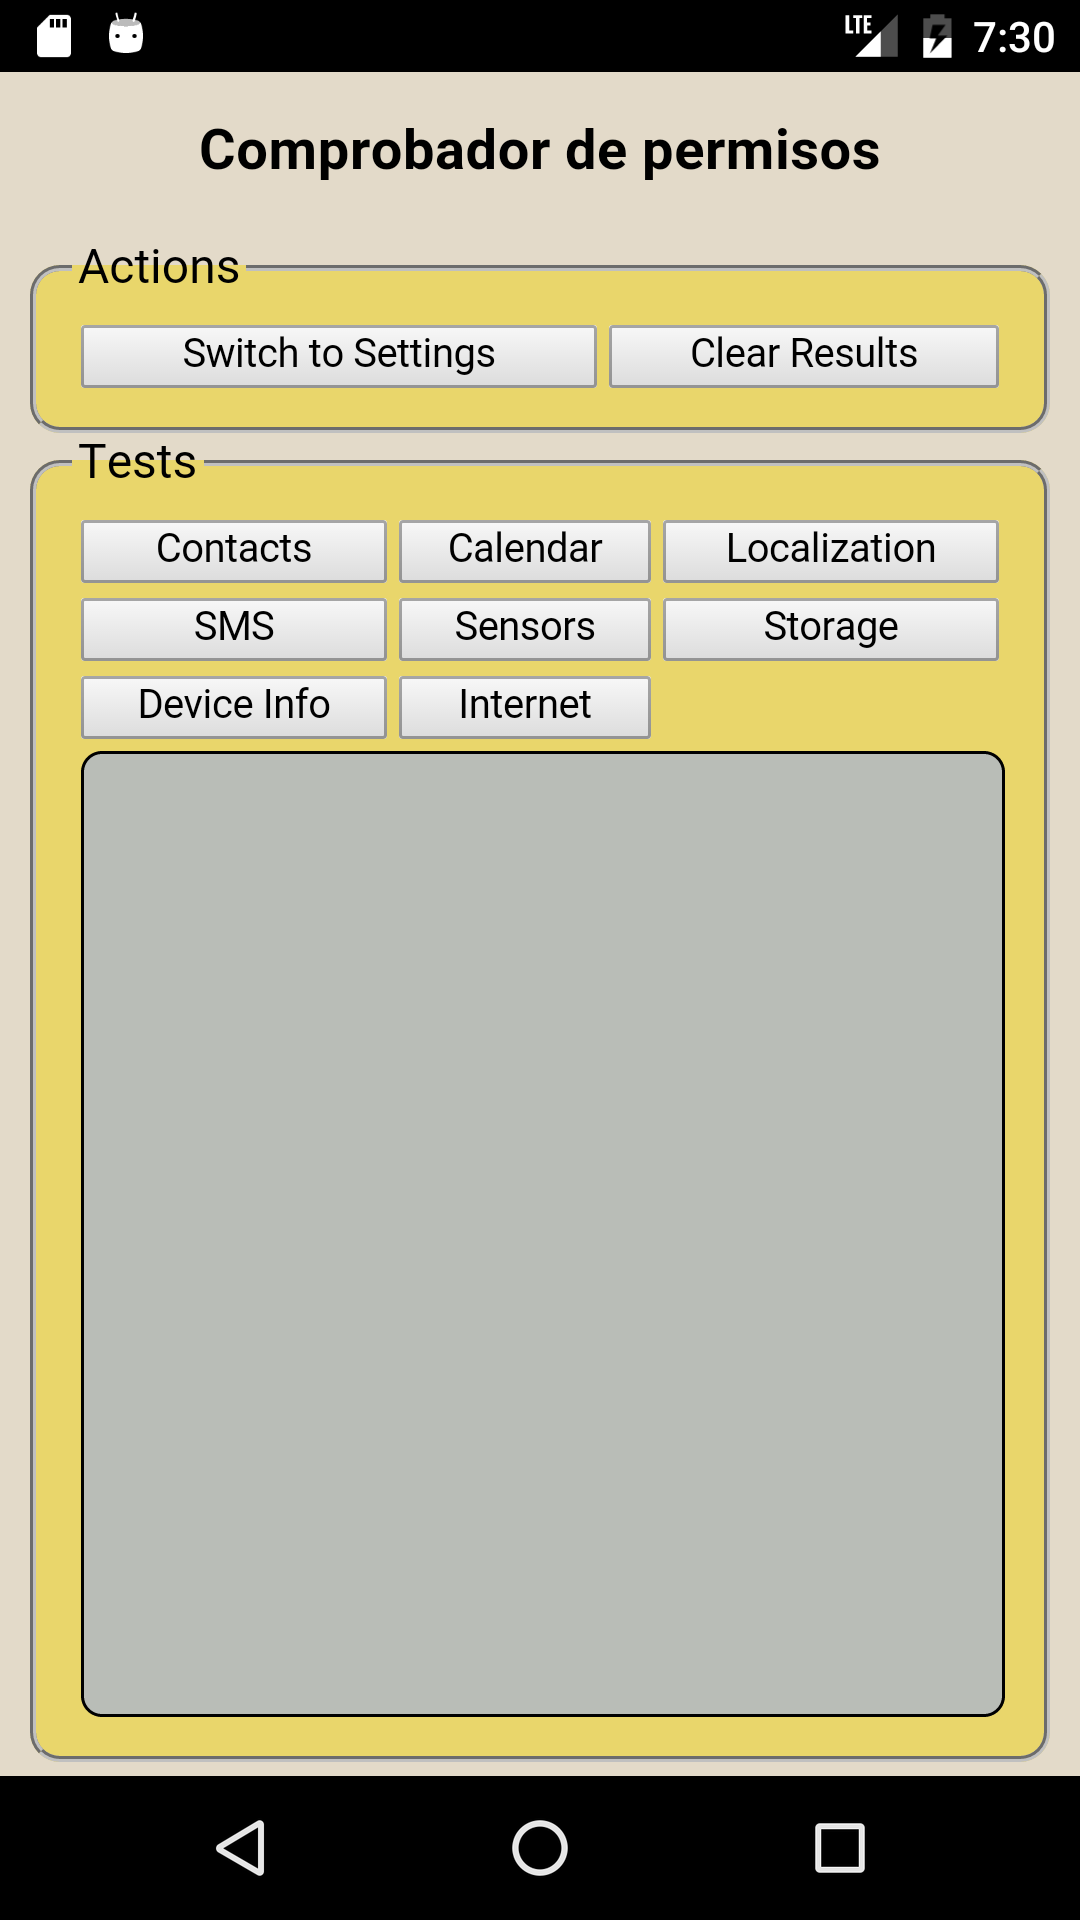
\includegraphics[width=0.4\linewidth]{chapter5/app_main_view}
	\caption{Áreas de la aplicación \textit{Runtime Permissions Test}.}
	\label{fig:chapter05:main_view}
\end{figure}
Mientras que la segunda área se subdivide en dos: en la parte de los tests y la parte de la consola. Una parte corresponde a los botones de los tests que, al presionarse, ejecutan el respectivo test, mostrando en la consola el resultado. Dicho resultado se mostrara con tipografía color verde si fue exitoso; en cambio, se mostrara con tipografía color roja de ser fallido.\\
A continuación se mencionan los componentes que se pueden testear con el framework:
\begin{itemize}
	\item Contactos
	\item Calendario
	\item Geolocalización
	\item SMS
	\item Sensores
	\item Almacenamiento
	\item Información del dispositivo.
	\item Acceso a Internet
\end{itemize}
\subsection{Funciones no compatibles}
El emulador ofical de Android es compatible con la mayoría de las funciones de un dispositivo, pero no incluye la posibilidad de virtualizar los siguientes componentes \cite{daemu}:
\begin{itemize}
    \item WiFi;
    \item Bluetooth;
    \item NFC\footnote{Del ingles \emph{Near Field Communication}. Es una tecnología de comunicación inalámbrica, de corto alcance y alta frecuencia que permite el intercambio de datos entre dispositivos.};
    \item Manipulación de la tarjeta SD;
    \item Conexión USB;
    \item Micrófono;
    \item Cámara
\end{itemize}
Al no poder manipular la tarjeta SD, no es posible testear ninguna las funcionalidades multimedia: no se pueden grabar audio, ni video ni sacar fotos.\\
Por lo tanto, no se agregaron al framework tests para los componentes listados anteriormente.
\section{Cátalogo de test}
En esta sección se listaran todos los test que conforman al framework. Para cada test se detalla su algoritmo, los plugins de Apache Cordova que se utilizaron para desarrollarlo y una serie de capturas que muestran los casos exitosos y fallidos.\\
Para acceder al panel de configuraciones, se utilizo el siguiente plugin:\\ \href{https://www.npmjs.com/package/cordova.plugins.diagnostic}{cordova.plugins.diagnostic v3.1.7}
\subsection{Contactos}
El test consiste en crear un contacto y luego listar todos los contactos presentes en el dispositivo. En caso de ser exitoso, se muestran los contactos. De lo contrario, se muestra un error.\\
\begin{algorithm}
	\begin{algorithmic}[1]
		\STATE Se listan todos los contactos en la consola.
		\STATE Se crea un nuevo contacto.
		\STATE Se vuelven a listar todos los contactos en la consola.
	\end{algorithmic}
	\caption{Test de Contactos.}\label{alg:chap5:test_contactos}
\end{algorithm}
\textbf{\emph{Plugin:}} \href{https://www.npmjs.com/package/cordova-plugin-contacts}{cordova-plugin-contacts v2.2.1}
\begin{figure}[hbtp]
    \centering
    \begin{subfigure}{0.3\linewidth}
        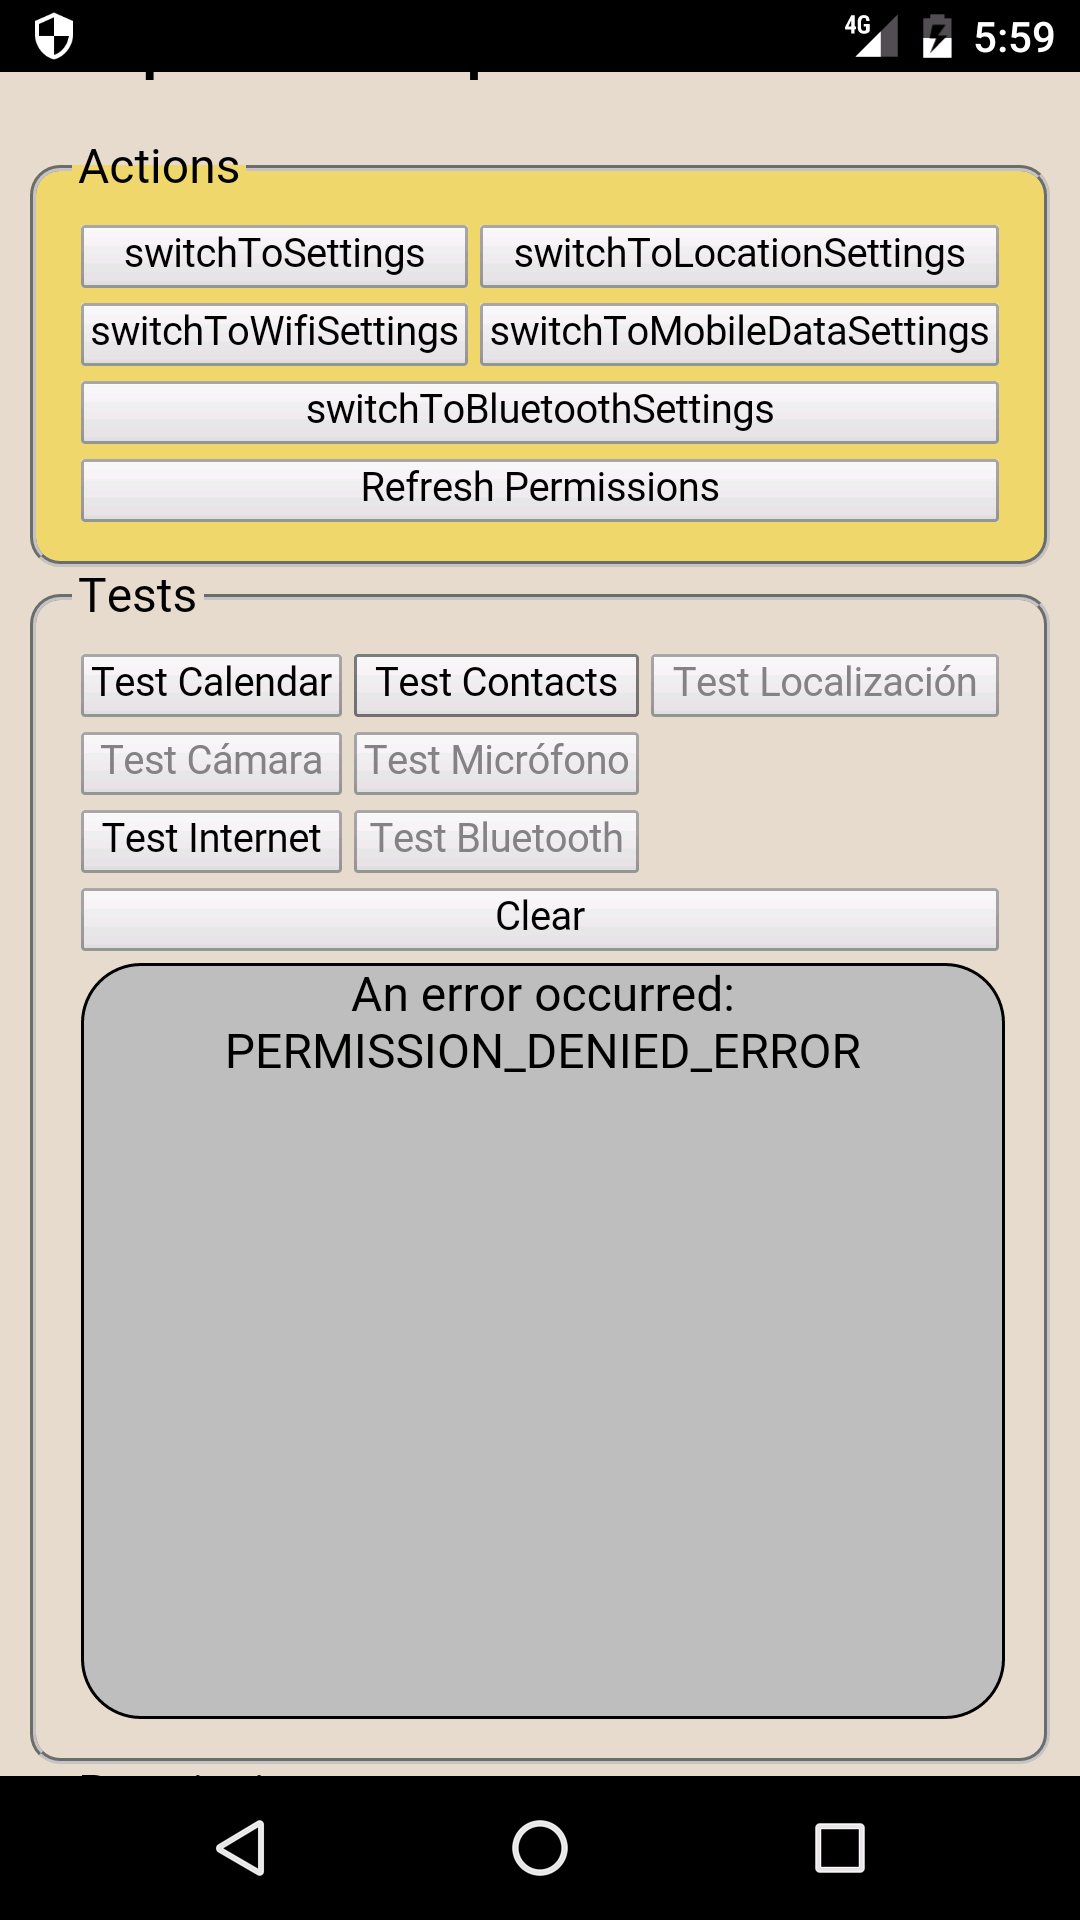
\includegraphics[width=\linewidth]{chapter5/without_contact}
        \label{fig:chapter05:without_contact}
    \end{subfigure}
    \begin{subfigure}{0.3\linewidth}
        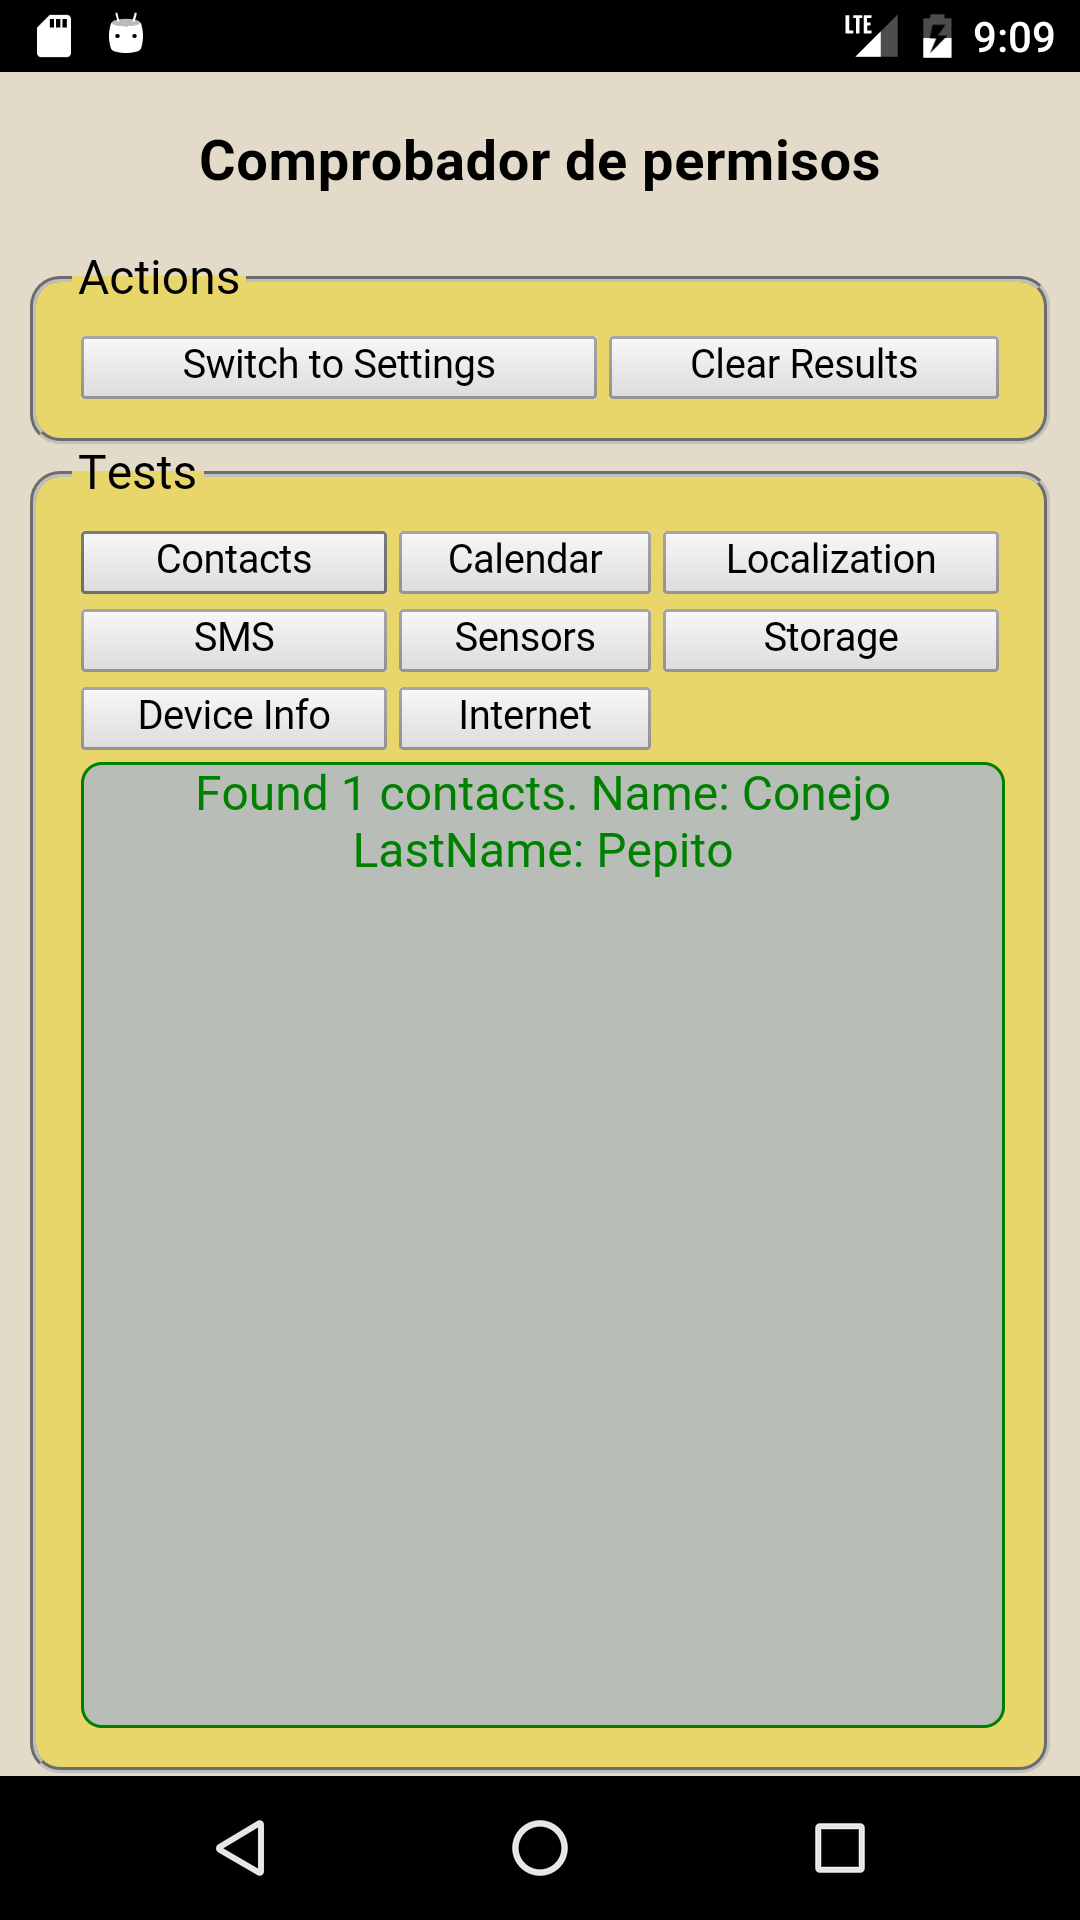
\includegraphics[width=\linewidth]{chapter5/with_contact}
        \label{fig:chapter05:with_contact}
    \end{subfigure}
    \caption{Testeando la administración de los contactos.}
	\label{fig:ch05:contacts-cases}
\end{figure}
\newpage
\subsection{Calendario}
El test consiste en crear un evento en un determinado rango de fechas y luego listar todos los eventos dentro del rango. En caso de ser exitoso, se muestran los datos del evento. De lo contrario, se muestra un error.\\
\begin{algorithm}
	\begin{algorithmic}[1]
		\STATE Se crean las fechas $startDate$ y $endDate$.
		\STATE Se crea un evento que empieza en la fecha $startDate$ y termina en la fecha $endDate$.
		\STATE Se listan en la consola los eventos entre las fechas $startDate$ y $endDate$.
	\end{algorithmic}
	\caption{Test del Calendario.}\label{alg:chap5:test_calendario}
\end{algorithm}
\textbf{\emph{Plugin:}} \href{https://www.npmjs.com/package/cordova-plugin-calendar}{cordova-plugin-calendar v4.5.5}
\begin{figure}[hbtp]
    \centering
    \begin{subfigure}{0.3\linewidth}
        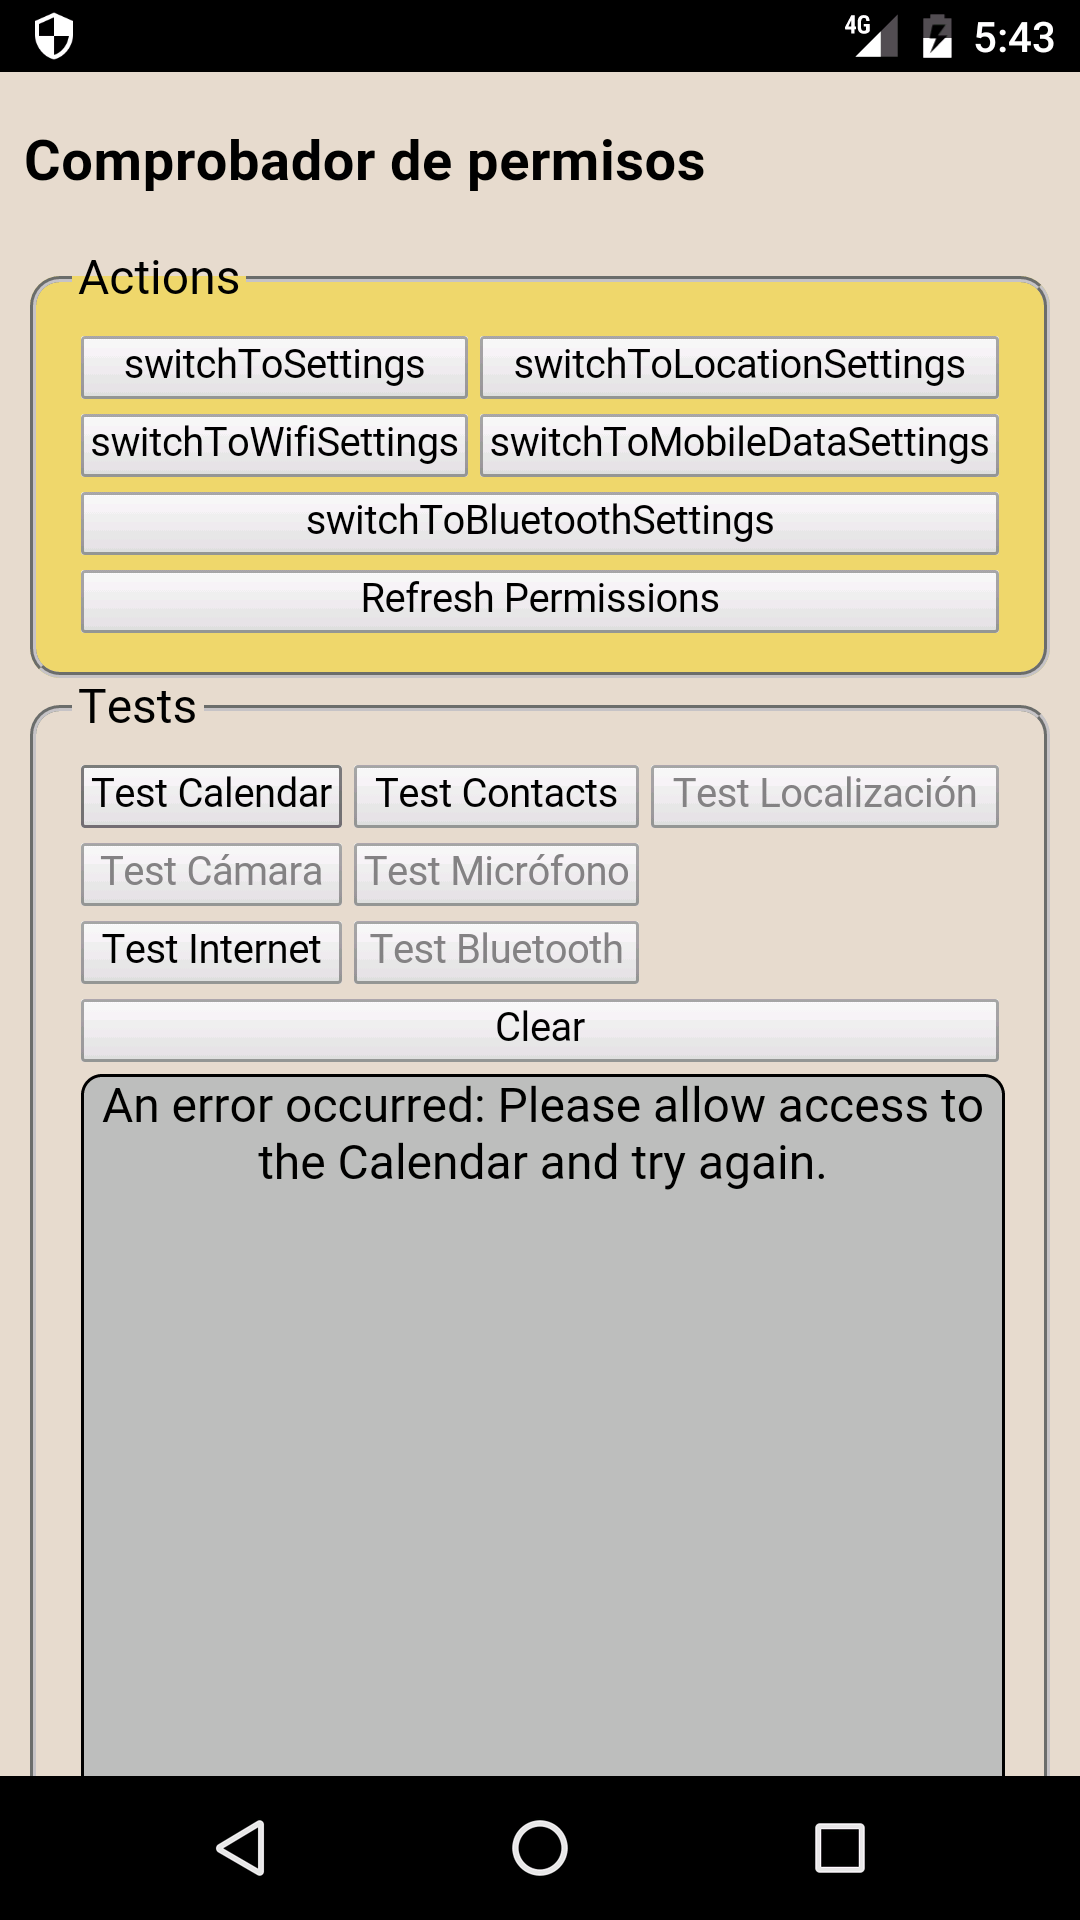
\includegraphics[width=\linewidth]{chapter5/without_calendar}
        \label{fig:ch05:without_calendar}
    \end{subfigure}
    \begin{subfigure}{0.3\linewidth}
        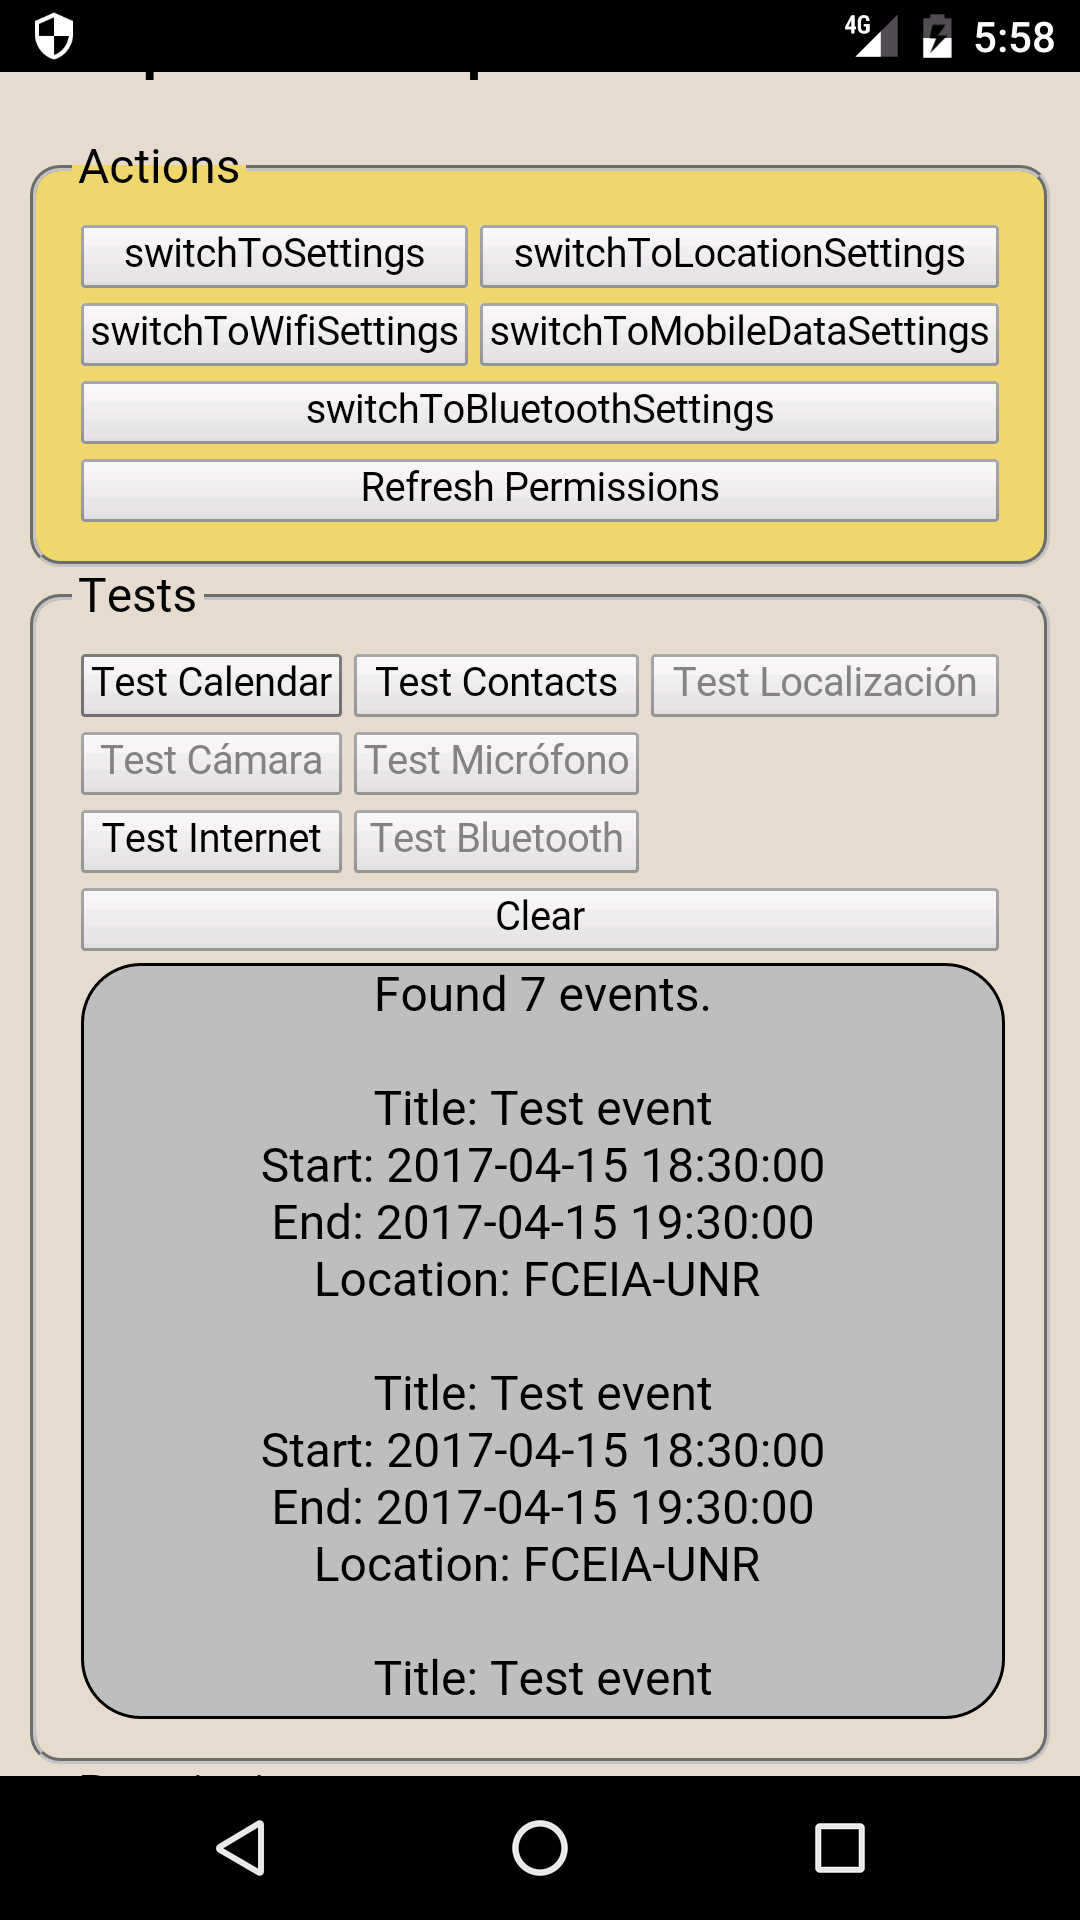
\includegraphics[width=\linewidth]{chapter5/with_calendar}
        \label{fig:ch05:with_calendar}
    \end{subfigure}
    \caption{Caso exitoso y caso fallido.}
	\label{fig:ch05:calendar-cases}
\end{figure}
\newpage
\subsection{Geolocalización}
Para realizar este test, se configuró el emulador de Android para que simule las coordenadas \texttt{(-122$^\circ$, 37$^\circ$)}, tal como se observa en la Figura \ref{fig:ch05:android_extended_controls}. Dicha configuración también se realizo en emulador oficial de iOS.\\
\begin{figure}[hbtp]
    \centering
	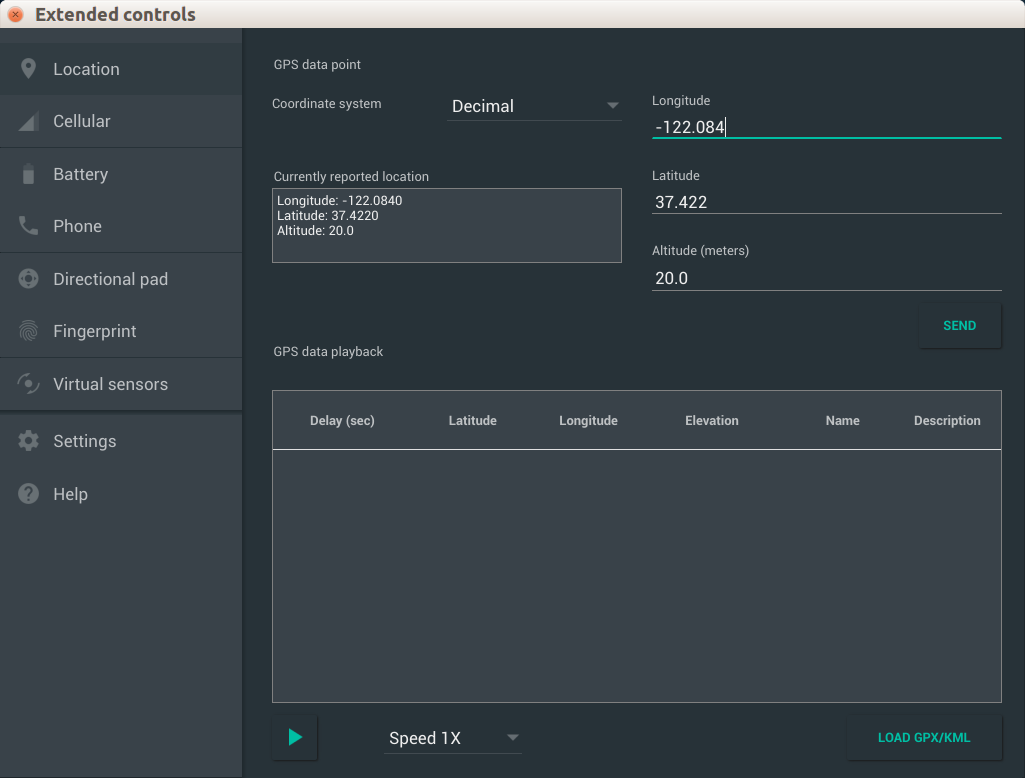
\includegraphics[width=0.6\linewidth]{chapter5/android_extended_controls}
	\caption{Panel de configuración de coordenadas del emulador de Android.}
	\label{fig:ch05:android_extended_controls}
\end{figure}
\begin{algorithm}
	\begin{algorithmic}[1]
		\STATE Se censa el GPS.
		\STATE Se muestran los datos en la consola.
	\end{algorithmic}
	\caption{Test de Geolocalización.}\label{alg:chap5:test_geolocalizacion}
\end{algorithm}
\textbf{\emph{Plugin:}} \href{https://github.com/apache/cordova-plugin-geolocation}{cordova-plugin-geolocation v2.4.3}
\begin{figure}[hbtp]
    \centering
	\begin{subfigure}{0.3\linewidth}
		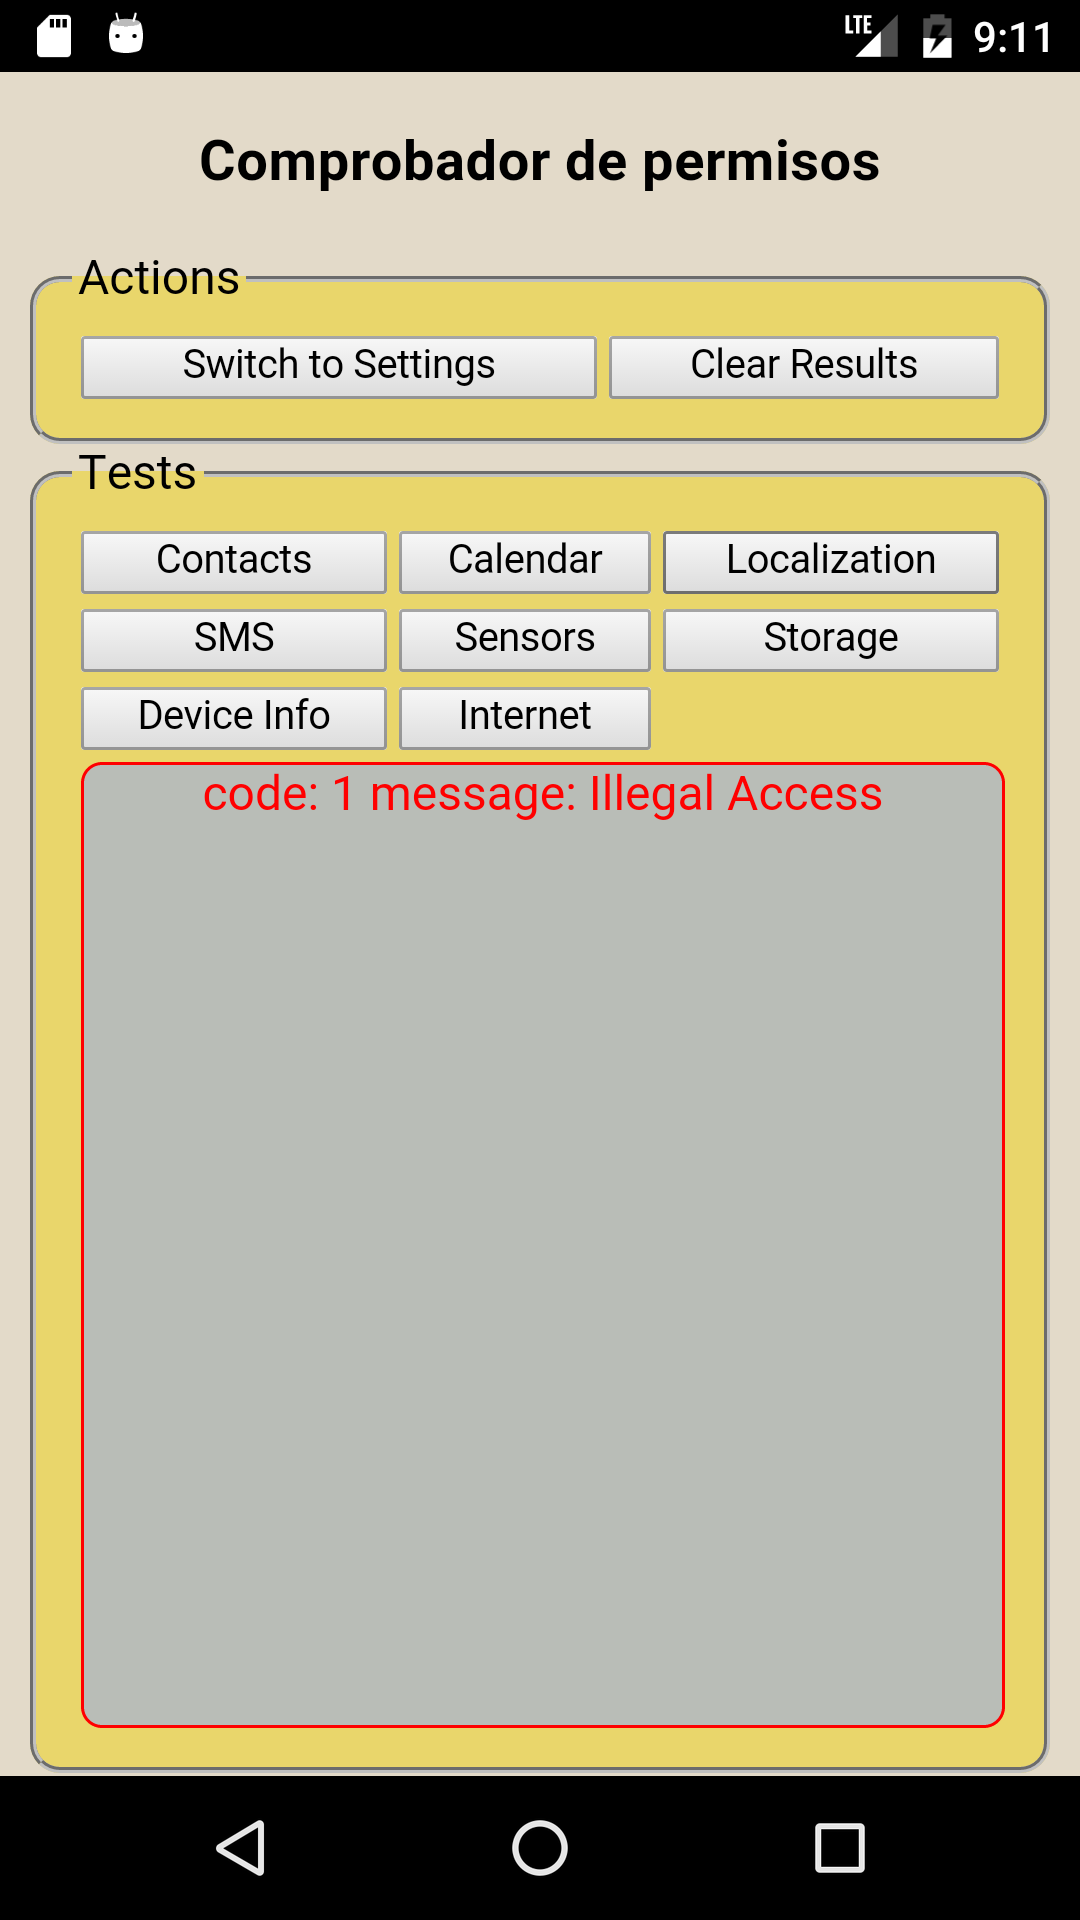
\includegraphics[width=\linewidth]{chapter5/without_location}
		\label{fig:ch05:without_location}
	\end{subfigure}
	\begin{subfigure}{0.3\linewidth}
		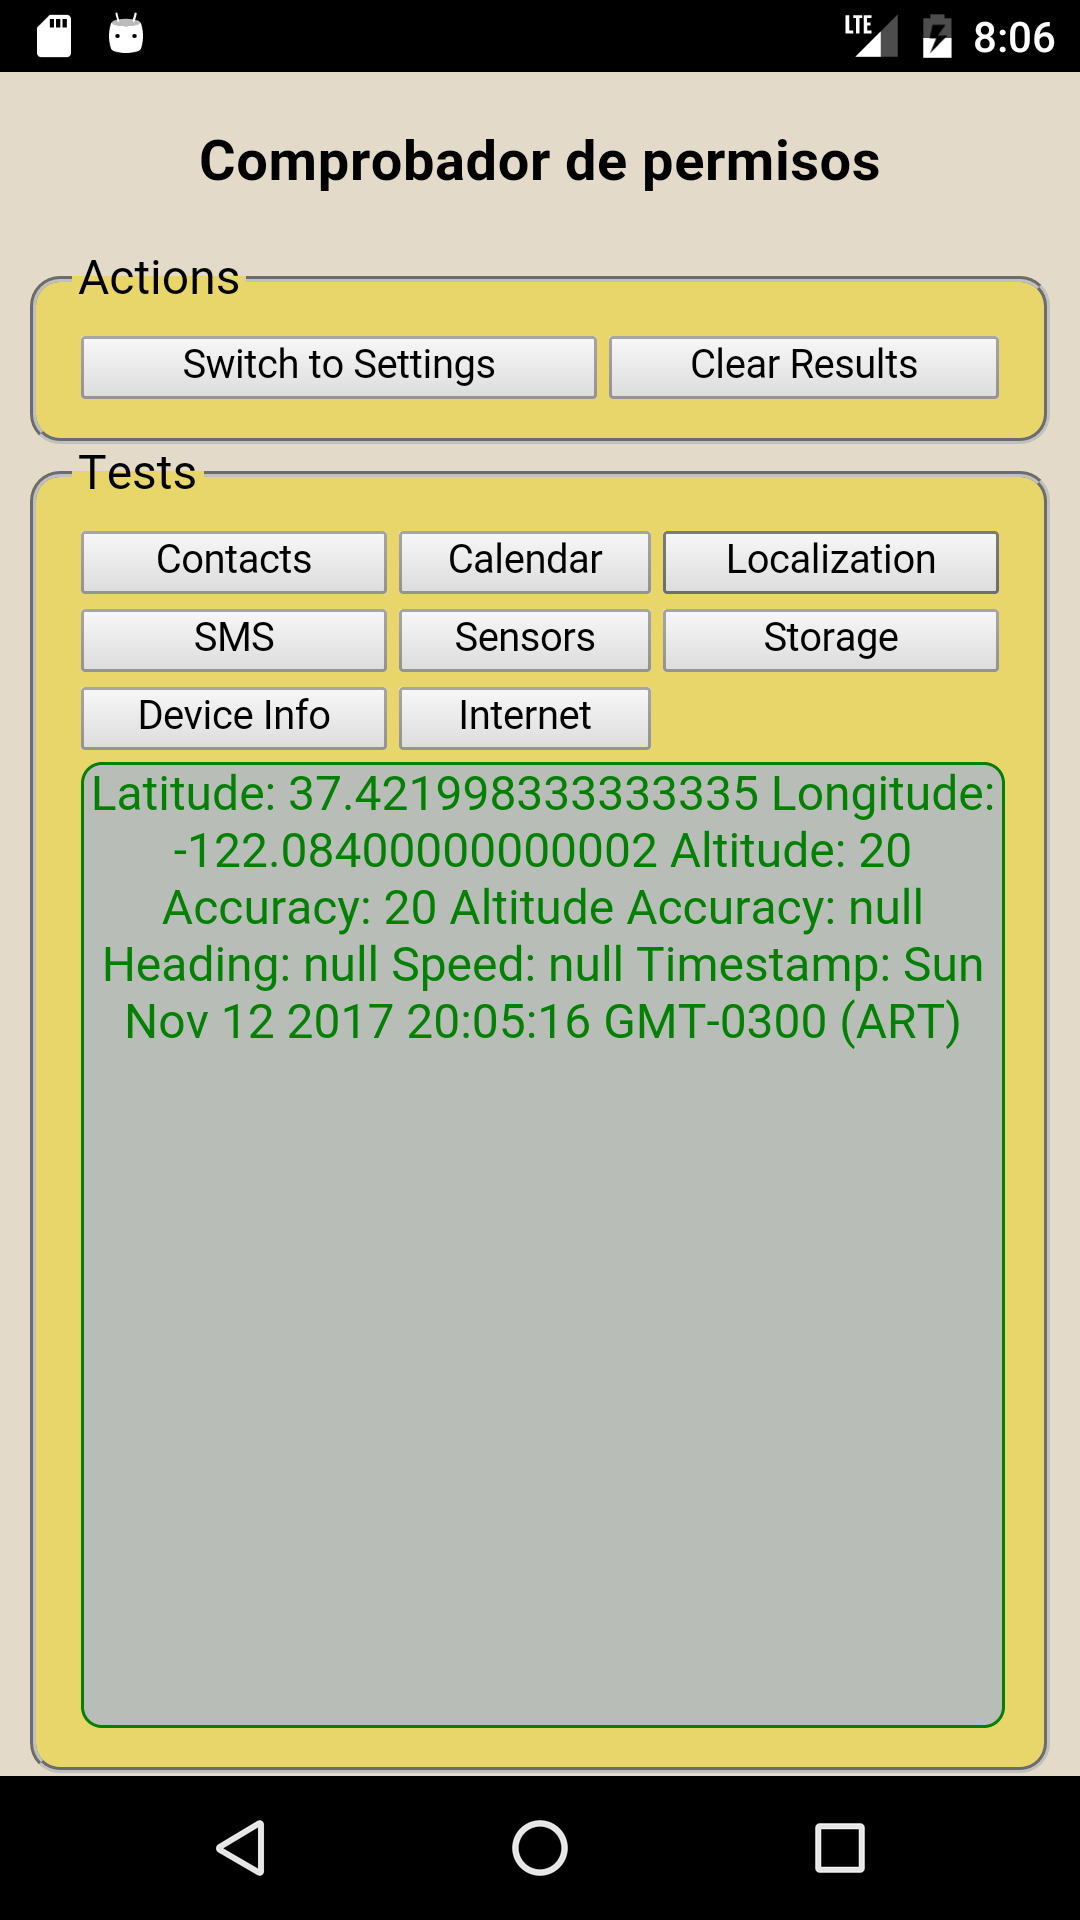
\includegraphics[width=\linewidth]{chapter5/location_success}
		\label{fig:ch05:with_location}
	\end{subfigure}
	\caption{Testeando la geolocalización.}
	\label{fig:ch05:geolocation-cases}
\end{figure}
\newpage
\subsection{SMS}
En un principio, se diseño un test con la capacidad de enviar mensajes, leerlos y recibirlos. Al momento de desarrollarlo, se encontró una restricción de seguridad en iOS: a partir de la version 8 no se pueden acceder a los mensajes SMS desde una aplicación instalada por el usuario \cite{foda, foda2}. En cambio, en Android si se pueden acceder, siempre que se tengan los permisos correspondientes.\\
Es por ello que se decidió quitar dicha funcionalidad, quedando disponible únicamente la posibilidad de enviar mensajes SMS.\\
\begin{algorithm}
	\begin{algorithmic}[1]
		\STATE Se inicializan los eventos para recibir SMS. 
		\STATE Se envía un SMS de prueba.
		\STATE Se indica el resultado del test en la consola.
	\end{algorithmic}
	\caption{Test de SMS.}\label{alg:chap5_test_sms}
\end{algorithm}
\textbf{\emph{Plugin:}} \href{https://github.com/floatinghotpot/cordova-plugin-sms}{cordova-plugin-sms v.1}
\begin{figure}[hbtp]
    \centering
	\begin{subfigure}{.3\linewidth}
		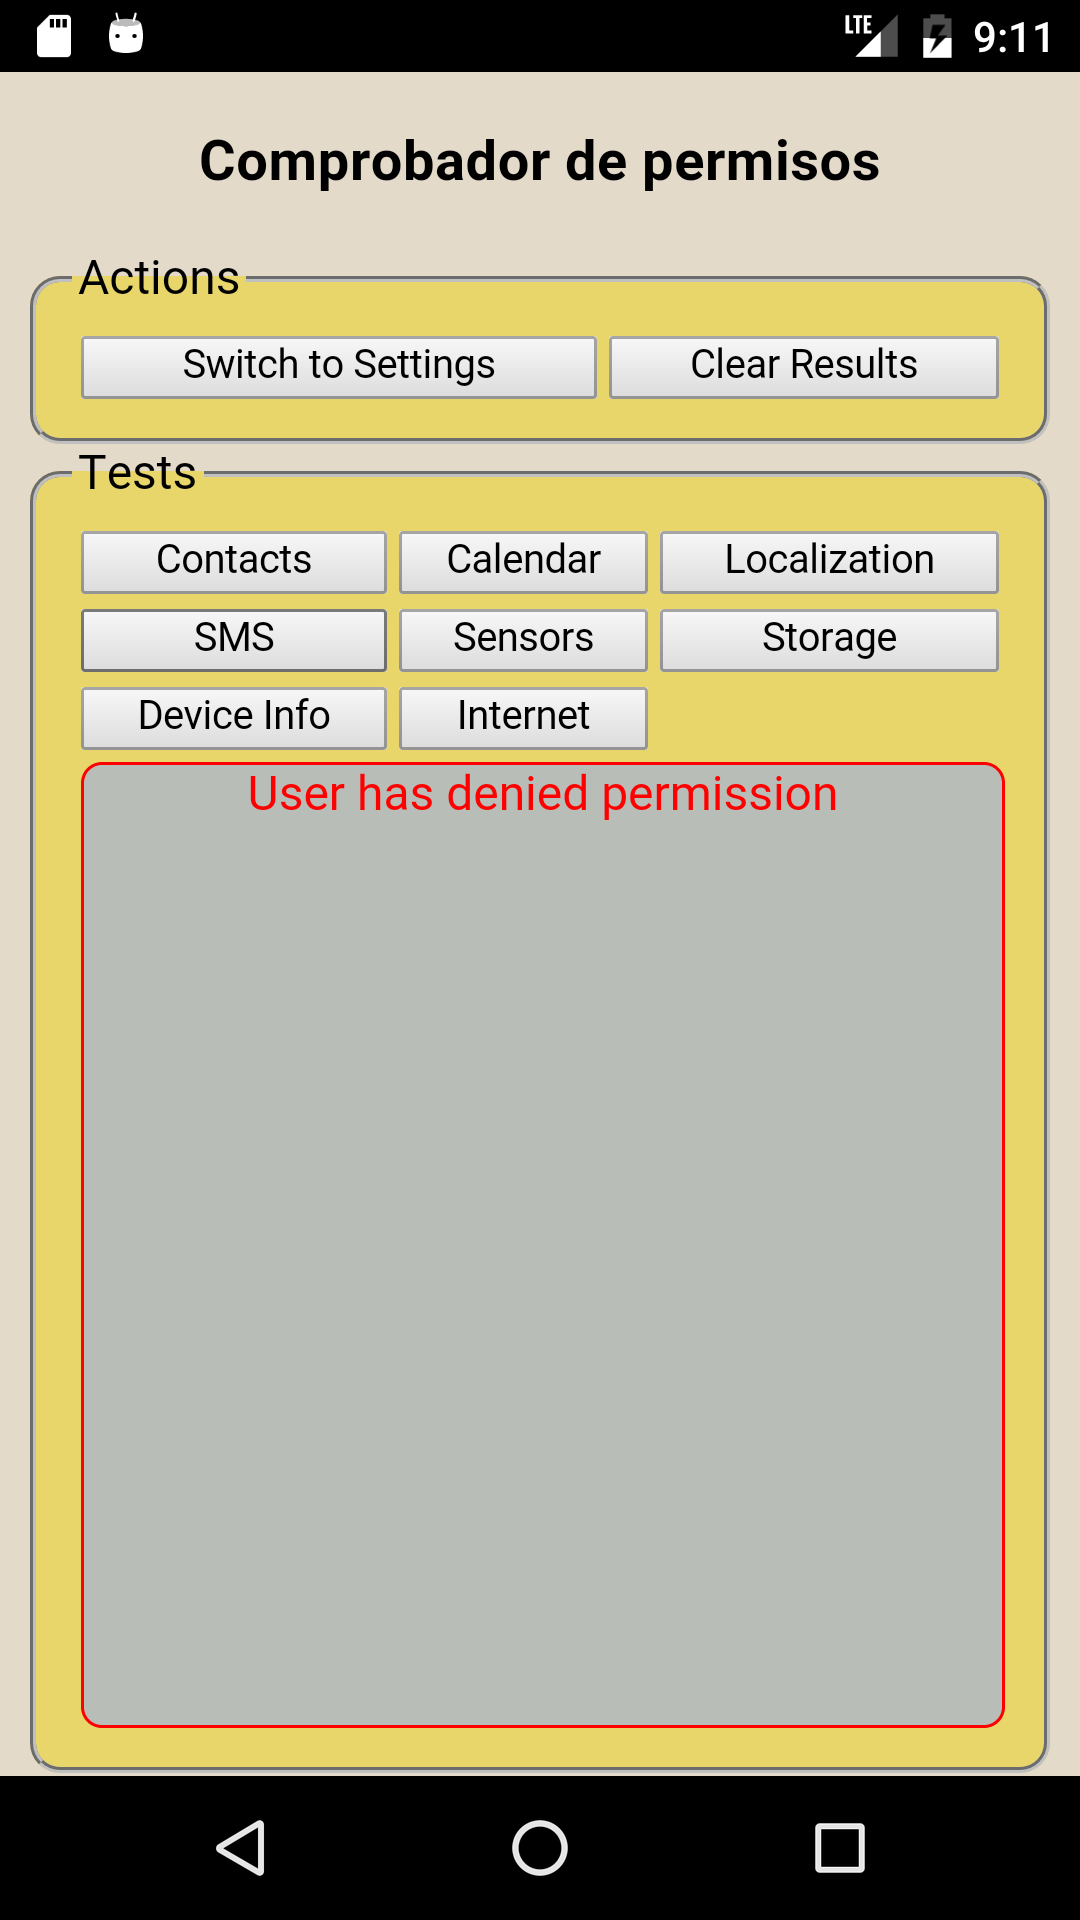
\includegraphics[width=\linewidth]{chapter5/without_sms}
		\label{fig:ch05:without_sms}
	\end{subfigure}
	\begin{subfigure}{.3\linewidth}
	    \centering
		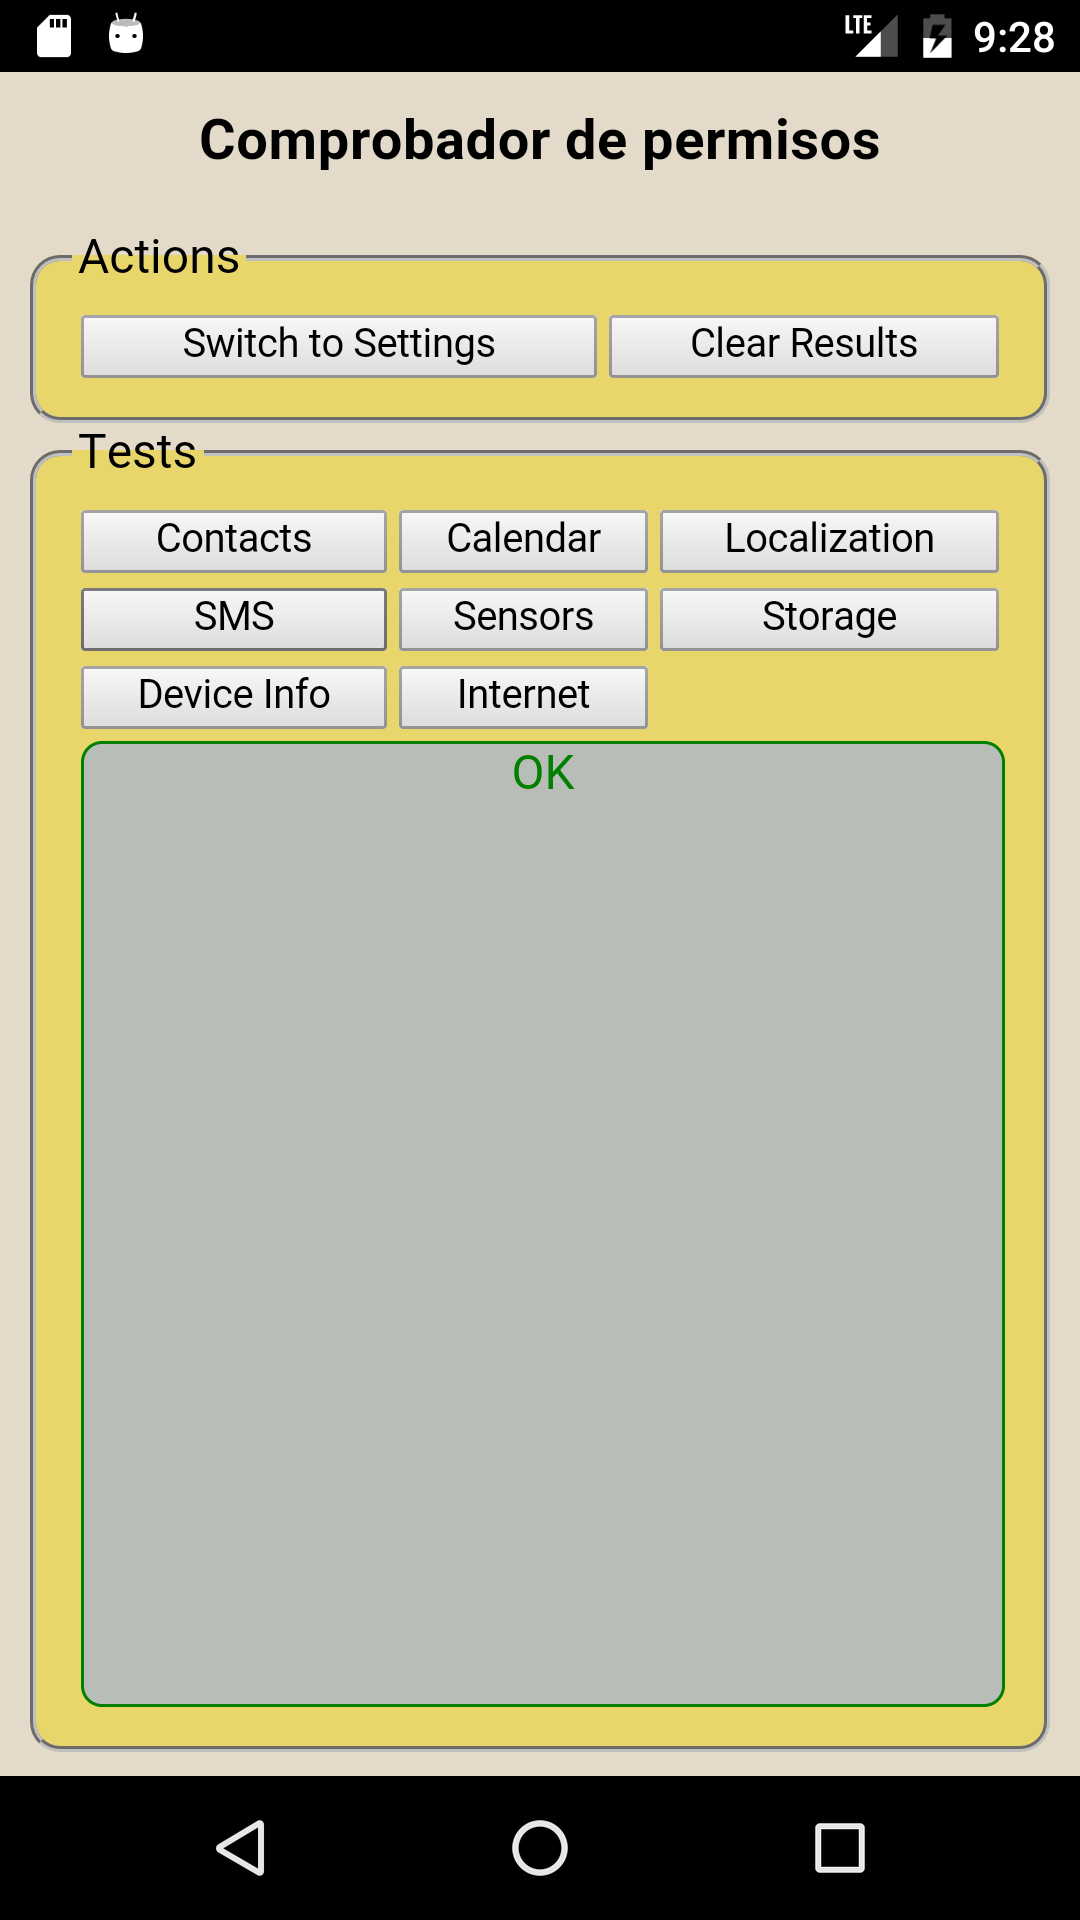
\includegraphics[width=\linewidth]{chapter5/success_sms}
		\label{fig:ch05:with_sms}
	\end{subfigure}
	\caption{Test de los permisos de los mensajes SMS.}
	\label{fig:chapter05:sms_test}
\end{figure}
\newpage
\subsection{Sensores}
El objetivo de este test es obtener datos de dos sensores del dispositivo: acelerómentro y giroscopio. Para ello, se configura un \texttt{timer}. Durante el tiempo que este activo, se tomaran distintos muestreos; y cuando ocurra el \emph{timeout} se mostrarán los datos en la consola de la aplicación.\\
\begin{algorithm}
	\begin{algorithmic}[1]
		\STATE Se inicializa un \texttt{timer} con \texttt{5 seg} para detener las mediciones.
		\STATE Se inicia la medición del acelerómentro.
		\STATE Se inicia la medición del giroscopio.
		\STATE Se muestran los resultados en la consola.
	\end{algorithmic}
	\caption{Test de los Sensores.}\label{alg:chap5_test_sensors}
\end{algorithm}
\textbf{\emph{Plugin:}} \href{https://www.npmjs.com/package/cordova-plugin-device-motion}{cordova-plugin-device-motion}\\
\textbf{\emph{Plugin:}} \href{https://www.npmjs.com/package/cordova-plugin-gyroscope}{cordova-plugin-gyroscope}\\
\begin{figure}[hbtp]
    \centering
	\begin{subfigure}{.3\linewidth}
	    \centering
		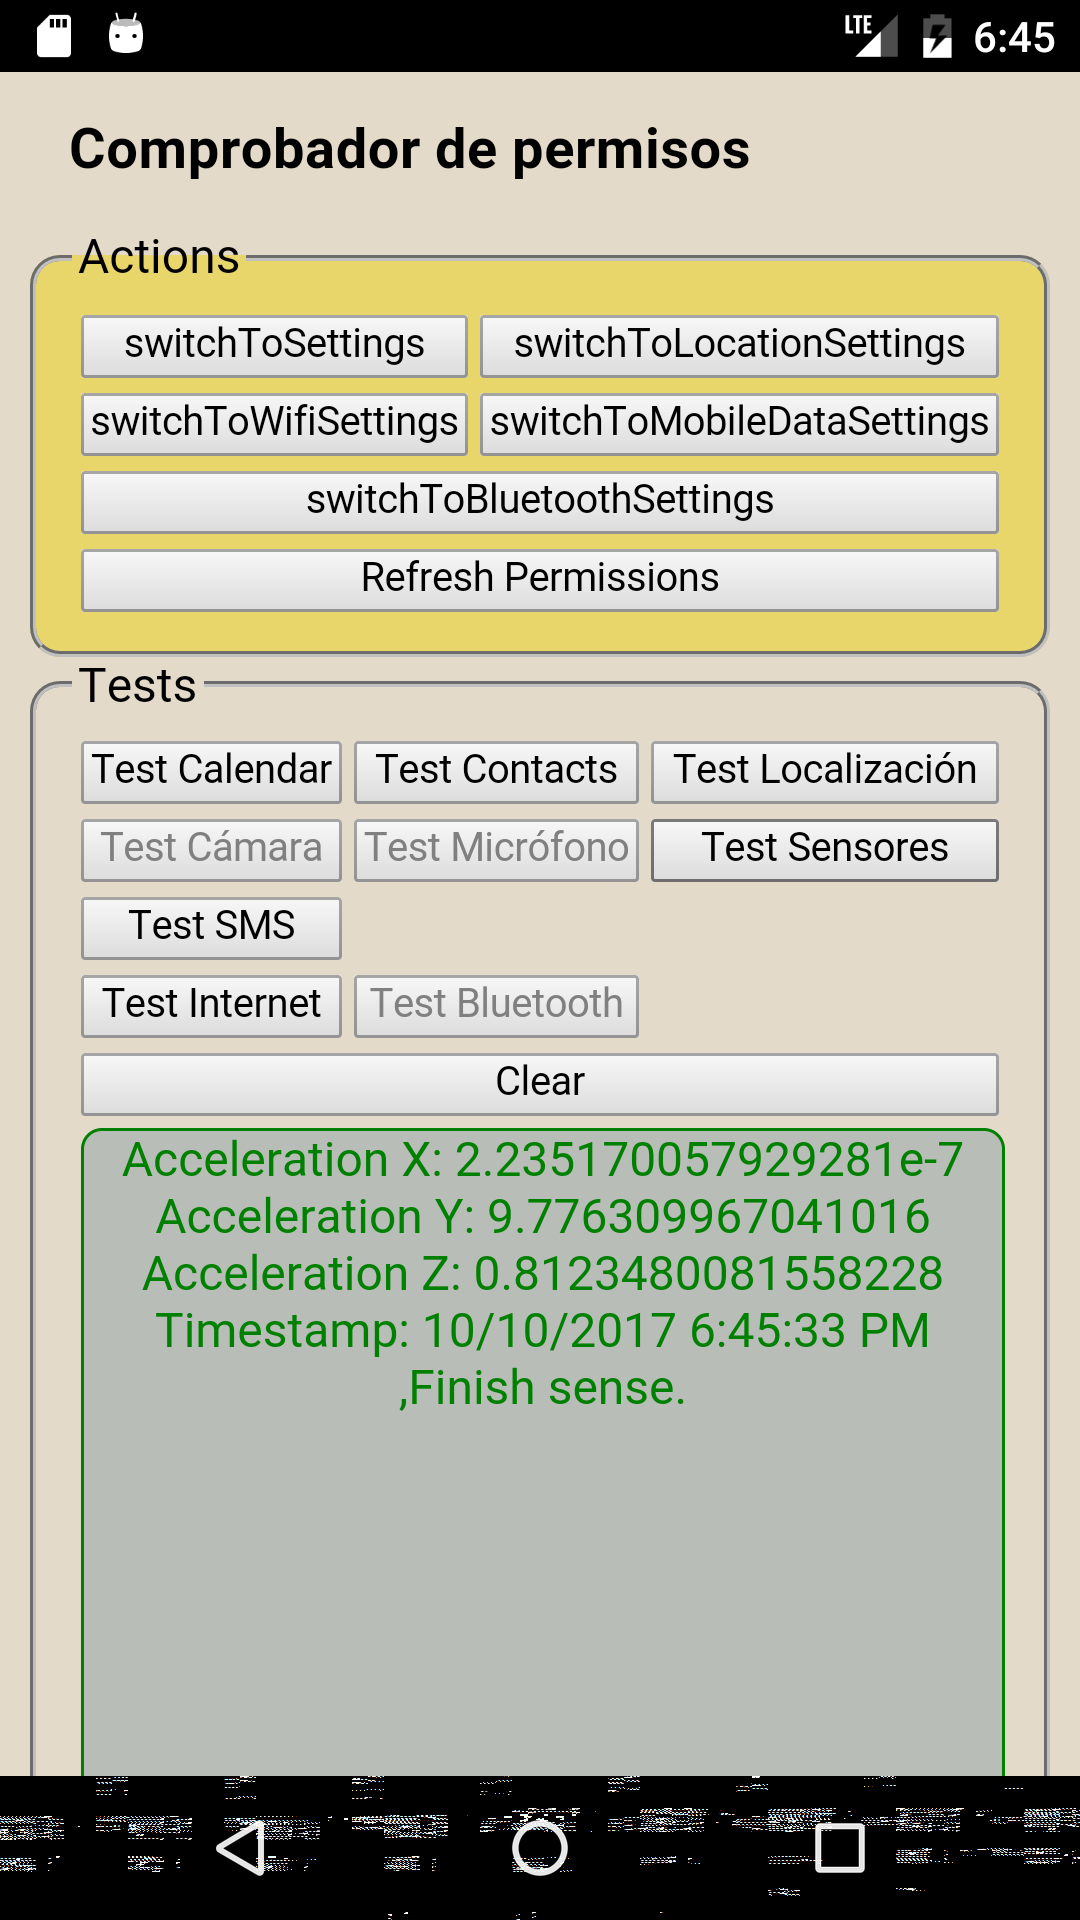
\includegraphics[width=\linewidth]{chapter5/accelerometer_success}
		\label{fig:ch05:accelerometer_success}
	\end{subfigure}
	\caption{Datos medidos.}
	\label{fig:chapter05:sensors_test}
\end{figure}
En iOS no fueron necesarios permisos para poder correr el test.
\newpage
\subsection{Almacenamiento}
El presente test fue diseñado para probar el alcance de los permisos de escritura sobre el sistema de archivos que tiene cada plataforma.\\
\begin{algorithm}
	\begin{algorithmic}[1]
		\STATE Se intenta capturar la pantalla.
		\STATE Se guarda la captura en el dispositivo.
		
	\end{algorithmic}
	\caption{Test de Almacenamiento.}\label{alg:chap5_test_storage}
\end{algorithm}
\textbf{\emph{Plugin:}} \href{https://github.com/gitawego/cordova-screenshot}{cordova-screenshot}\\
\begin{figure}[hbtp]
   \centering
   	\begin{subfigure}{.3\linewidth}
		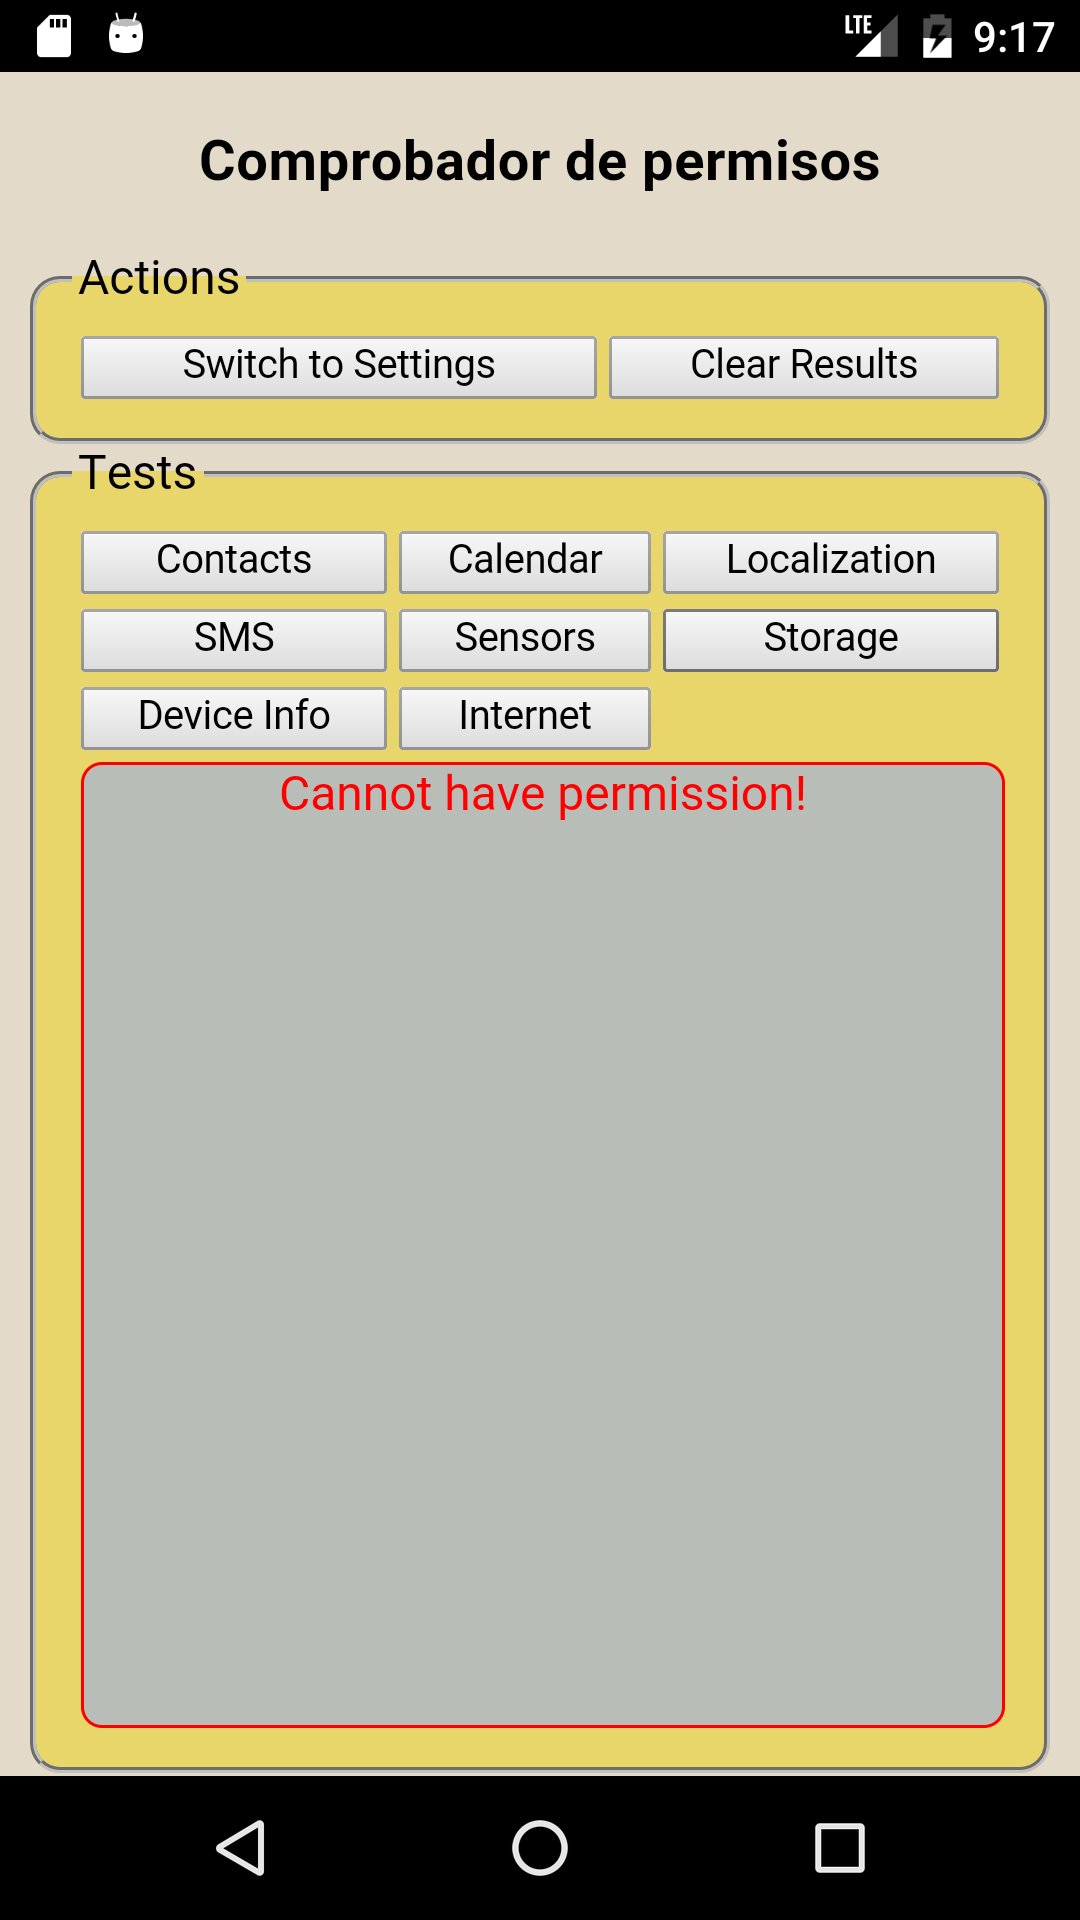
\includegraphics[width=\linewidth]{chapter5/storage_fail}
		\label{fig:ch05:storage_fail}
	\end{subfigure}
	\begin{subfigure}{.3\linewidth}
		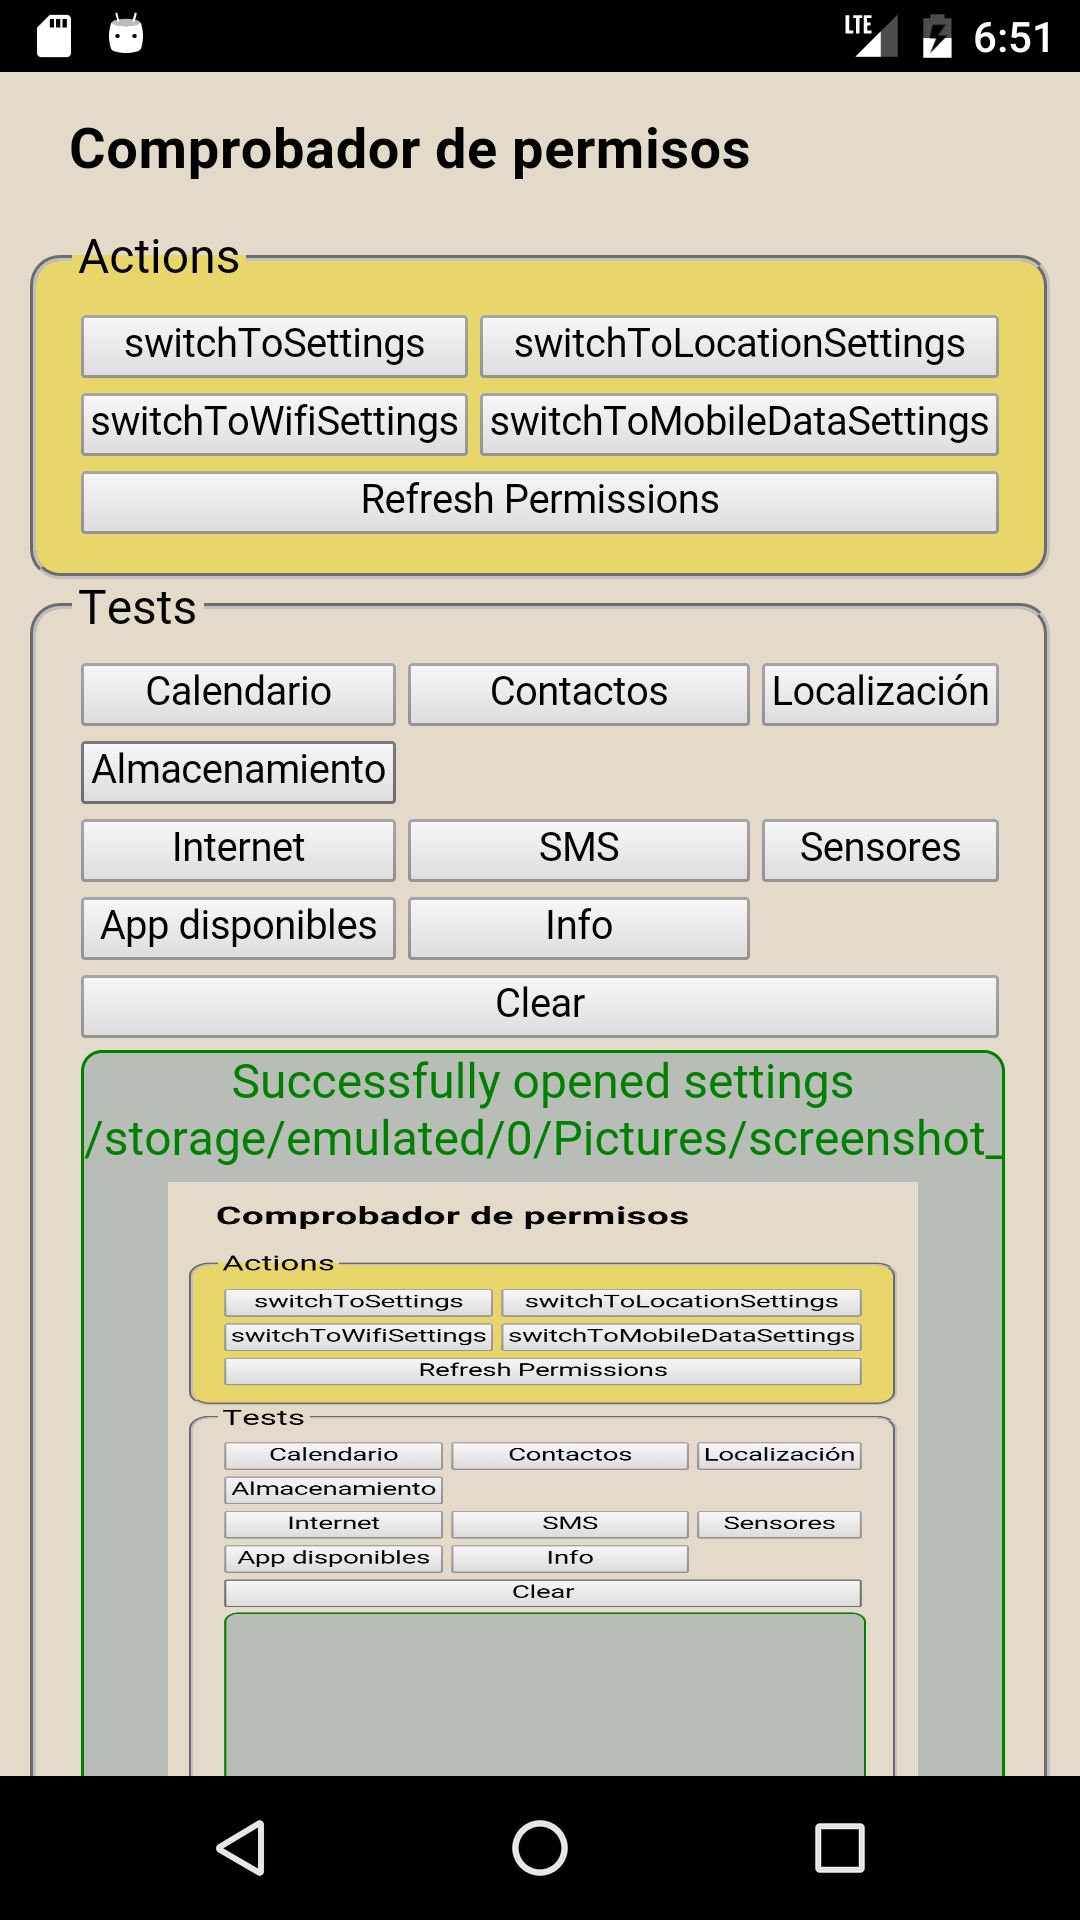
\includegraphics[width=\linewidth]{chapter5/storage_success}
		\label{fig:ch05:storage_success}
	\end{subfigure}
	\caption{Testeando el almacenamiento en el dispositivo.}
	\label{fig:ch05:storage_test}
\end{figure}
En iOS no fueron necesarios permisos para poder correr el test.
\newpage
\subsection{DeviceInfo}
El objetivo de este test es obtener datos del dispositivo donde corre la aplicación: plataforma, modelo, serial, entre otros.\\
\begin{algorithm}
	\begin{algorithmic}[1]
		\STATE Se obtienen los datos del dispositivo.
		\STATE Se muestra por consola los datos obtenidos.
	\end{algorithmic}
	\caption{Test de Informacion del Dispositivo.}\label{alg:chap5_test_info}
\end{algorithm}
\textbf{\emph{Plugin:}} \href{https://www.npmjs.com/package/cordova-plugin-device}{cordova-plugin-device}\\
\begin{figure}[hbtp]
   \centering
   	\begin{subfigure}{.3\linewidth}
		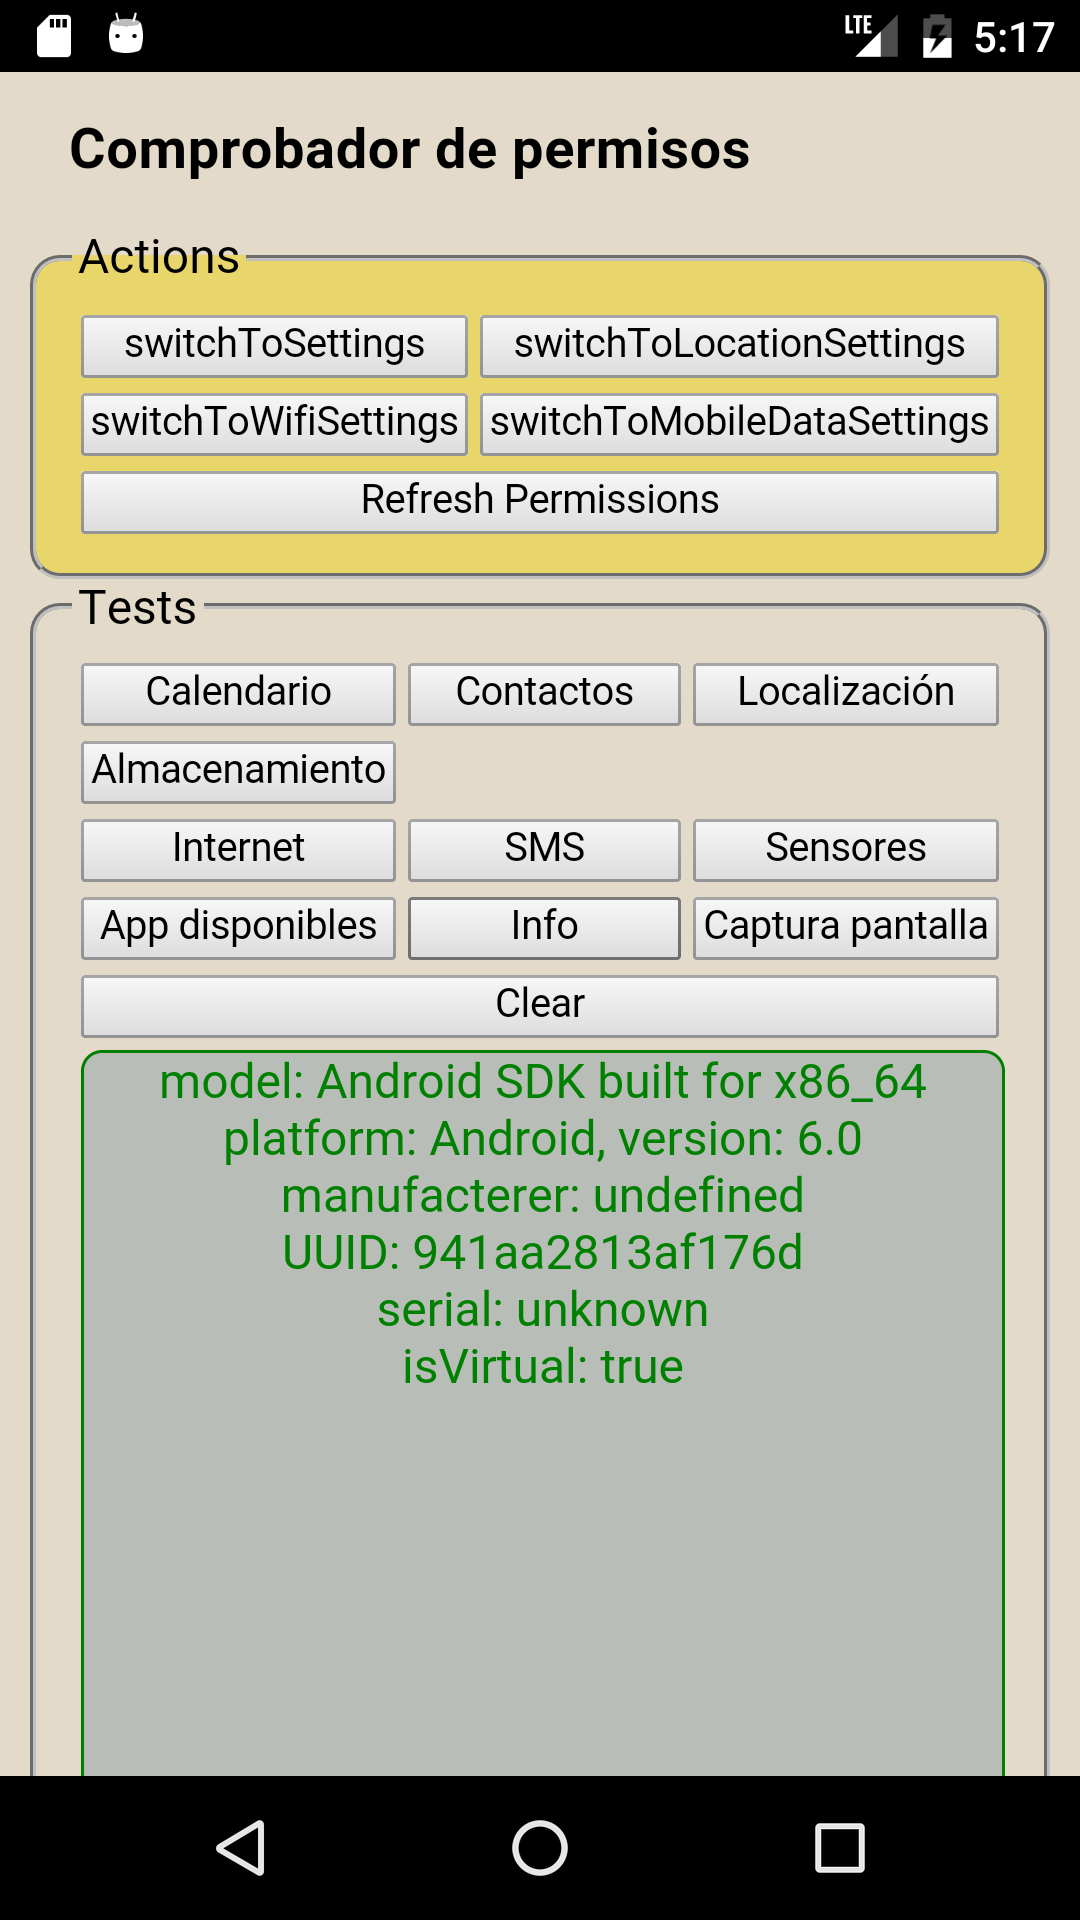
\includegraphics[width=\linewidth]{chapter5/device_info}
		\label{fig:ch05:device-info-success}
	\end{subfigure}
	\caption{Obteniendo datos del dispositivo.}
	\label{fig:ch05:device-info}
\end{figure}
No fueron necesarios permisos en ninguna de las dos plataformas para poder correr el test.
\newpage
\subsection{Internet}
El objetivo del presente test es establecer una comunicación a traves de Internet. No se requirió de ningún plugin para implementarlo.\\
La decodificación de la imagen se obtuvo de \href{https://stackoverflow.com/questions/19124701/get-image-using-jquery-ajax-and-decode-it-to-base64/25371174#25371174}{StackOverflow}. Al ejecutarse en un emulador, para probar el acceso a Internet, se habilitó/deshabilitó la Red Inalámbrica de la computadora donde se corrieron los emuladores.\\
\begin{algorithm}
	\begin{algorithmic}[1]
		\STATE Se realiza una consulta GET HTTP hacia \href{https://dcc.fceia.unr.edu.ar/sites/all/themes/birthofcool/images/logo-lcc.png}{logo del DCC}
		\STATE Se decodifica la imagen (viene codificada en Base64).
		\STATE Se muestra en consola un \texttt{tag} \textless IMG\textgreater, cuyo \texttt{source} es el dato decodificado.
		\STATE Se realiza una consulta POST HTTP hacia \href{http://httpbin.org/post}{httpbin}
		\STATE Se muestra en consola la respuesta.
	\end{algorithmic}
	\caption{Test de conexión a Internet.}\label{alg:chap5_test_internet}
\end{algorithm}
\begin{figure}[hbtp]
    \centering
    \begin{subfigure}{.3\linewidth}
		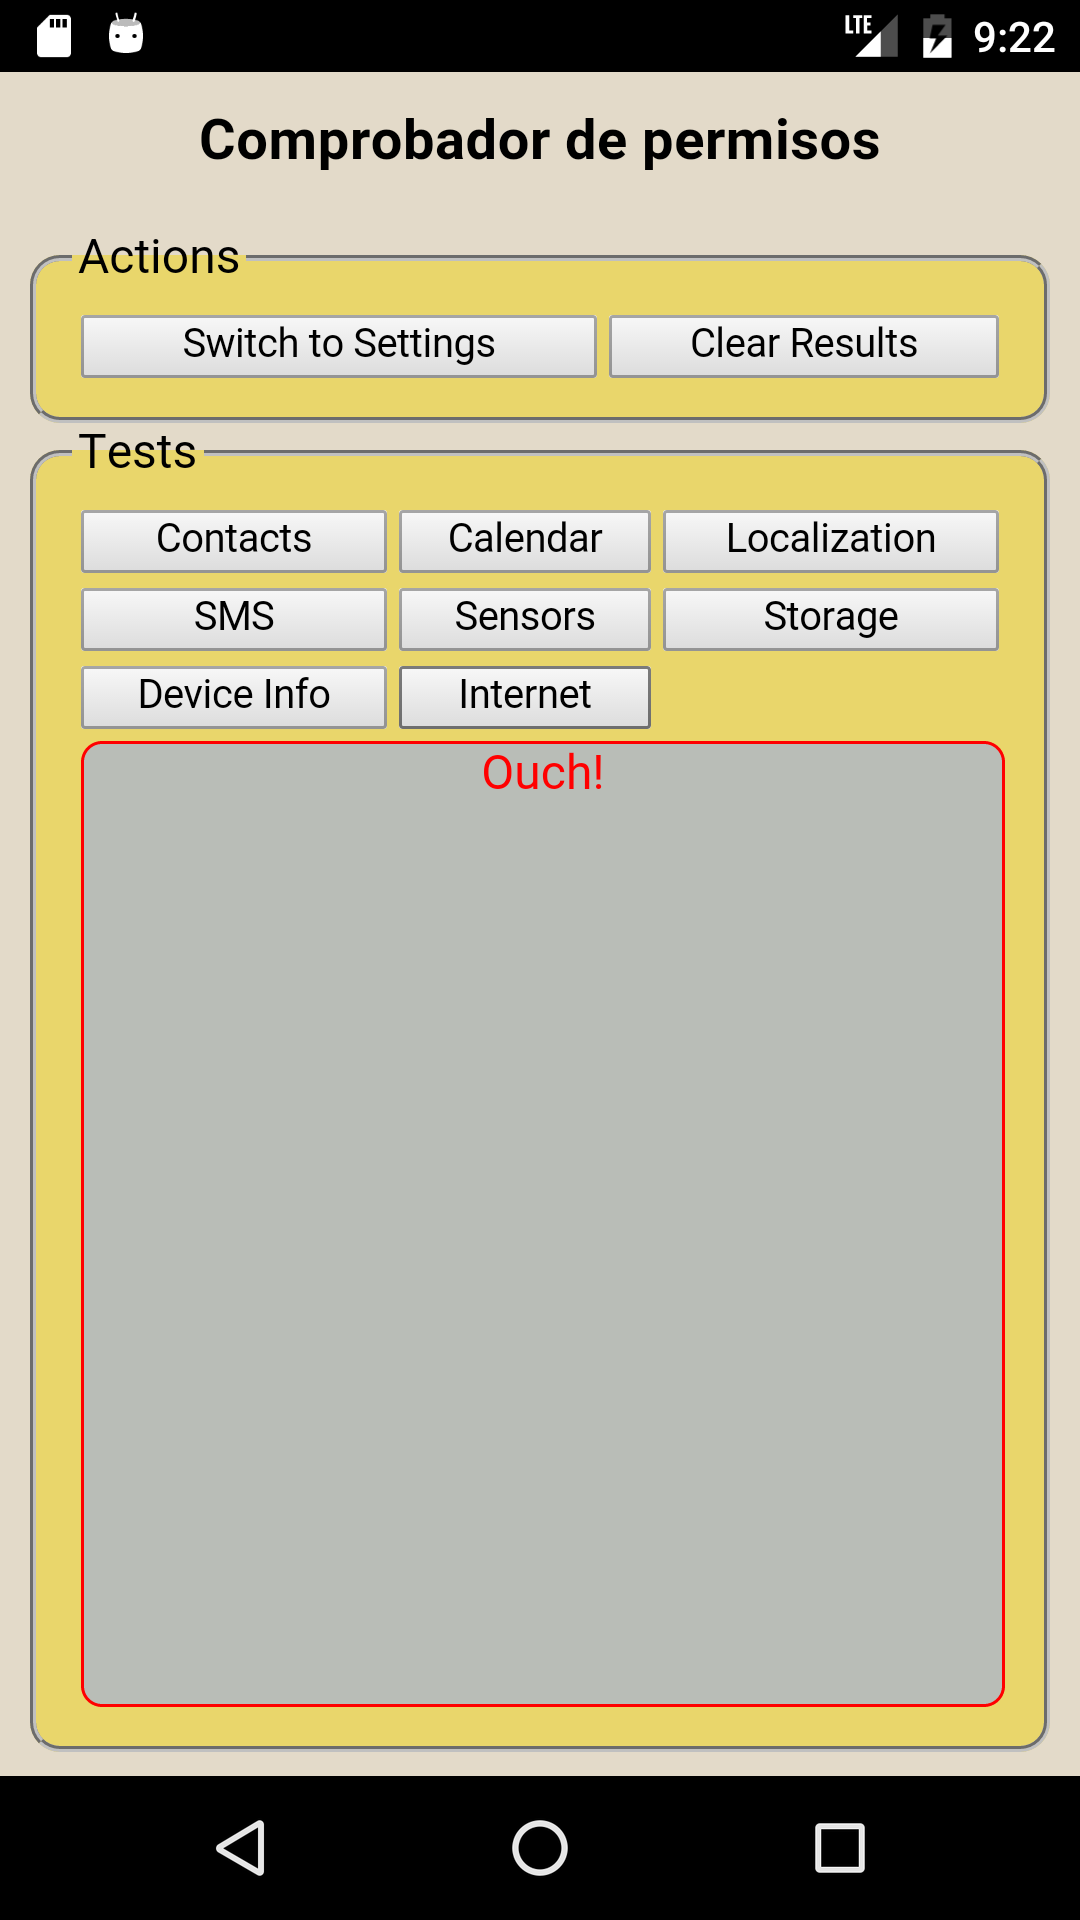
\includegraphics[width=\linewidth]{chapter5/fail_request}
		\label{fig:ch05:fail_request}
	\end{subfigure}
	\begin{subfigure}{.3\linewidth}
		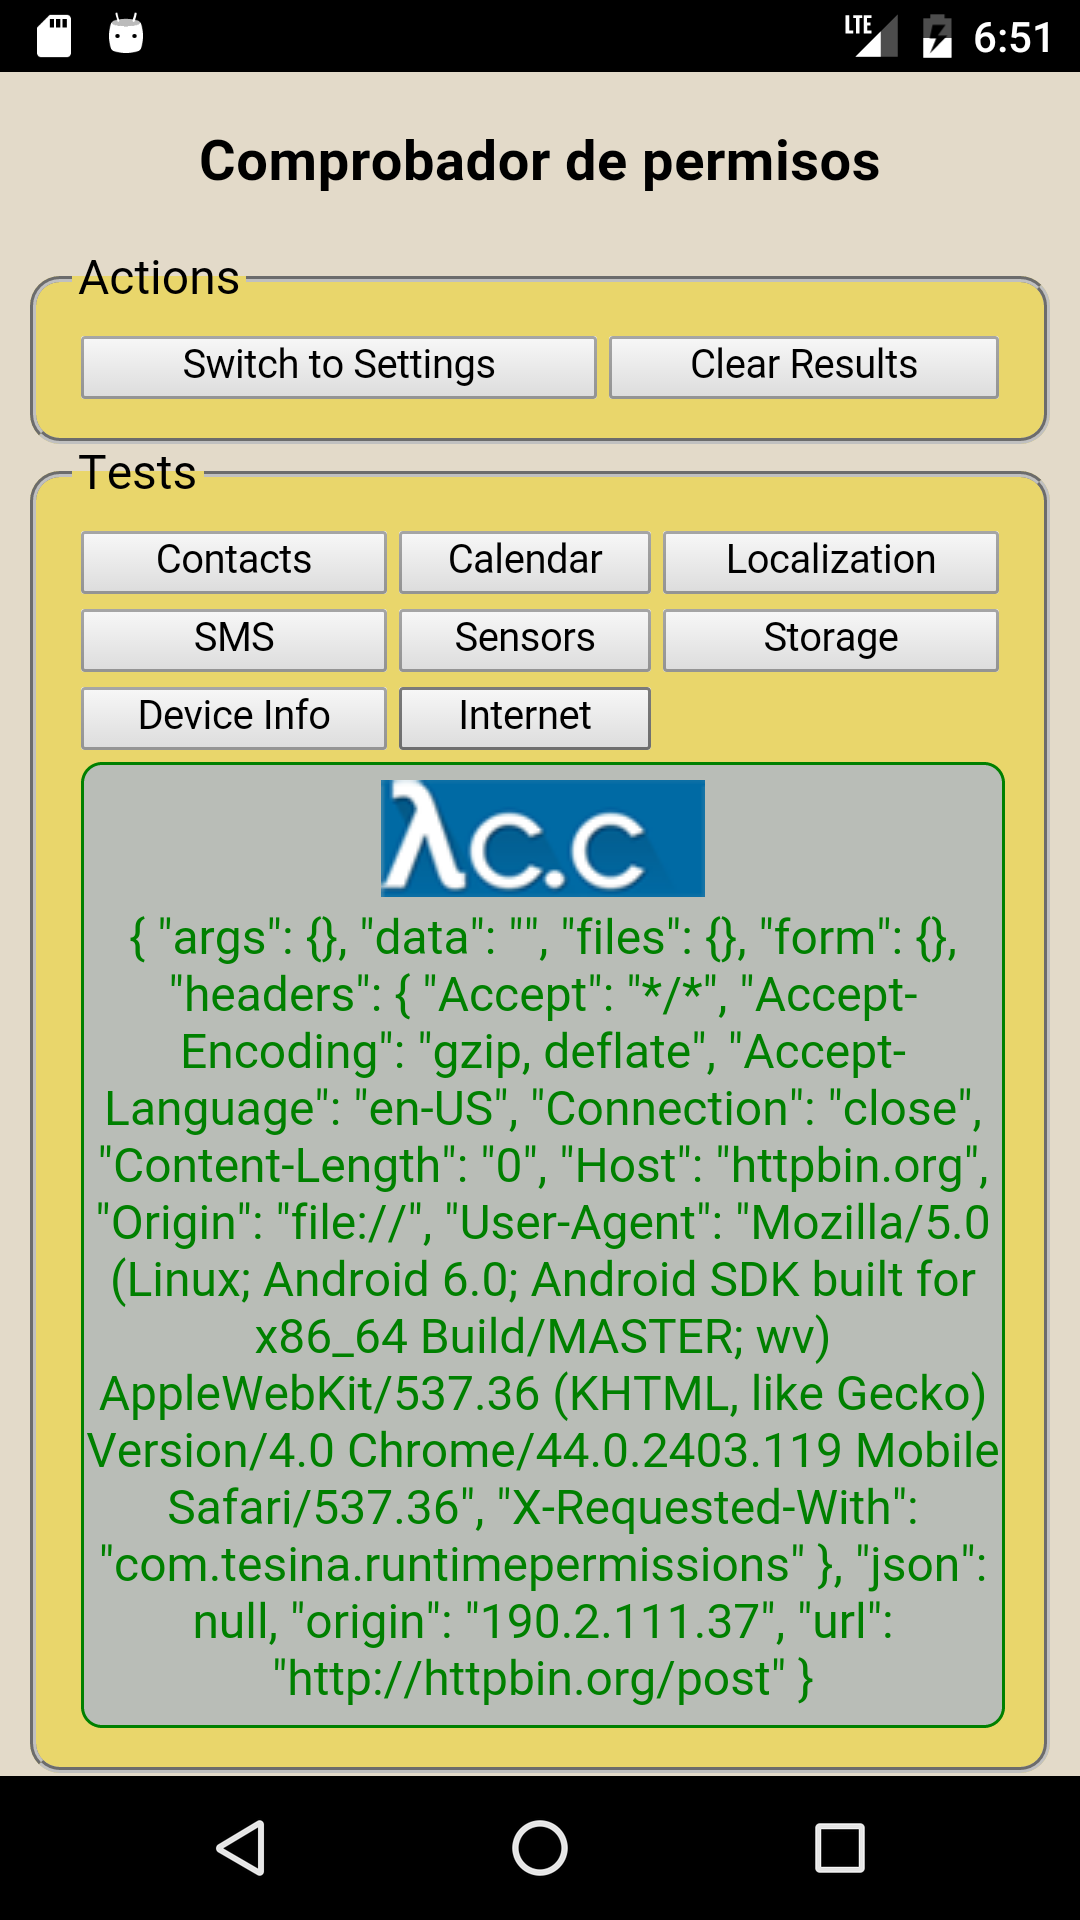
\includegraphics[width=\linewidth]{chapter5/success_request}
		\label{fig:ch05:success_request}
	\end{subfigure}
	\caption{Testeando el acceso a Internet.}
	\label{fig:ch05:internet_test}
\end{figure}
No fueron necesarios permisos en ninguna de las dos plataformas para poder correr el test.
\newpage
\section{Resultados experimentales}
El framework desarrollado en este trabajo tiene la capacidad de testear los componentes \emph{Contactos}, \emph{Calendario}, \emph{Geolocalización}, \emph{SMS}, \emph{Sensores}, \emph{Almacenamiento}, \emph{Información del dispositivo} y \emph{Acceso a Internet}, tal como se describe en la sección \ref{sec:main-view}.\\
Un primer resultado es poder clasificar los componentes testeados en tres clases, según requieran explícitamente permisos para utilizarlos. Dichas clases son:
\begin{itemize}
    \item \underline{Clase A}: son requeridos en ambas plataformas;
    \item \underline{Clase B}: son requeridos en Android;
    \item \underline{Clase C}: no requieren permisos.
\end{itemize}
Luego de correr los tests, se confecciono la Tabla \ref{tab:ch03:permission-classification}.\\
\begin{table}[hbtp]
    \centering
	\begin{tabular}{c c c}
		\hline
		\multicolumn{3}{c}{\emph{\textbf{Permisos}}} \\
		\emph{Ambas plataformas} 	& \emph{Solo Android}	 & \emph{Sin permisos}\\ \hline \hline
    Contactos    & -    & -\\
    Calendario    & -    & -\\
    Geolocalización    & -    & -\\
    -    & SMS\tablefootnote{Aplica solamente al envío de mensajes.}    & -\\
    -    & Sensores    & -\\
    -    & Almacenamiento    & -\\
    -    & -    & Información del dispositivo.\\
    -    & -    & Acceso a Internet\\ \hline \hline
	\end{tabular}
	\caption{Clasificación de permisos según si requieren autorización.}
	\label{tab:ch03:permission-classification}
\end{table}
\subsection{Clase A}
Los componentes que conforman esta clase son \emph{Contactos}, \emph{Calendario} y \emph{Geolocalización}. La característica común entre ellos es que requieren autorización explicita del usuario para interactuar con ellos. Sino se le concede el correspondiente permiso, no se puede acceder a ninguna funcionalidad del componente.\\
El primer componente a analizar es \emph{Contactos}. En Android, requiere el permiso \textit{peligroso} llamado Contacto y en iOS requiere el permiso llamado con el mismo nombre. En ambas plataformas, los dos permisos abarcan las mismas funcionales: permiten crear un contacto, borrarlo, editarlo y obtener un listado de todos los contactos presentes en el dispositivo.\\
Luego, se continua analizando el componente \emph{Calendario}. Permite administrar todo lo relacionado con los eventos: crear un evento, modificarlo y eliminarlo. Además, permite administrar varios calendarios. Cada evento esta relacionado a un calendario. En iOS, estas funcionalidades están separadas en dos componentes: \emph{Calendarios} y \emph{Recordatorios}. Cada uno de ellos tiene su permiso que lo regula. Sin embargo, el test solo prueba el uso del permiso llamado Recordatorios. Por otra parte, en Android el permiso \textit{peligroso} que regula estas funcionalidades se llama Calendario.\\
A continuación se analiza el último componente de esta clase, llamado \emph{Geolocalización}. En ambas plataformas, provee el acceso a la ubicación del dispositivo, ya sea la ubicación precisa (GPS) o la aproximada (WIFI/Móvil). Tanto en Android como en iOS, el permiso que regula dichas funcionalidades se llama Localización.\\
\subsection{Clase B}
Esta clase está compuesta por los componentes \emph{SMS}, \emph{Almacenamiento} y \emph{Sensores}. Ellos tienen en común es que para utilizar sus funcionalidades no requieren permisos en iOS. Sin embargo, necesitan autorización explicita en Android.\\
Se comenzara el análisis por el componente \emph{SMS}. Sus funcionalidades son: enviar un mensaje, eliminarlo, obtener los mensajes entrantes y obtener la lista de todos los mensajes, ya sean recibidos o enviados. Sin embargo, el test que se desarrolló solamente prueba el envío de mensajes, ya que iOS, a partir de la version 8, no se permite acceder al resto de las funcionalidades desde una aplicación de terceros (es decir, no nativa) \cite{foda, foda2}. En cambio, Android permite acceder a todas las funcionalidades mencionadas; y se pueden acceder a traves del permiso \textit{peligroso} llamado SMS.\\
Luego, se continua con el componente \emph{Sensores}. Dicho componente controla el acceso a los sensores del dispositivo. El test recolecta datos de dos sensores: el acelerómentro y el giroscopio. En Android, el permiso \textit{peligroso} que los regula se llama Sensores. Sin dicho permiso, no se pueden leer los datos de ningún sensor. En cambio, si se obtiene la autorización, se dispondrá de los datos de todos los sensores.\\
Finalmente, se hablara sobre el componente \emph{Almacenamiento}. En Android, el permiso que regula al componente mencionado tiene su mismo nombre. Dicho permiso resguarda las funcionalidades que permiten leer y escribir la tarjeta SD. En el test, se intenta escribir en el sistema de archivos.
\subsection{Clase C}
El objetivo de esta clase es agrupar componentes que tienen permisos \textit{normales} en Android. A pesar de ello, pueden ser potencialmente peligrosos a la hora de ser utilizados para violar la privacidad de un usuario. De todos los componentes que tienen relacionados algún permiso \textit{normal}, se eligieron dos: \emph{Información del dispositivo} y \emph{Acceso a Internet}. Cabe aclarar que ambos no requieren autorización explicita del usuario, en ninguna de las dos plataformas, para utilizar las funcionalidades que brindan.\\
El primer componente nos brinda datos relacionados al dispositivo en el cual se esta corriendo la aplicación. Especifica el modelo del dispositivo, el cual es establecido por el fabricante del dispositivo y puede ser diferente en todas las versiones del mismo producto. También se puede obtener información relacionada a la plataforma del dispositivo: nombre, versión, quién lo manufacturó, su UUID\footnote{Del ingles Universally Unique Identifier. Es un numero de 128 bits que identifica al dispositivo biunívocamente.} y si es emulado o no.\\
El segundo componente de esta clase es el que nos provee acceso a Internet. En la actualidad, son muchas las aplicaciones móviles que lo utilizan Internet. Según el ranking confeccionado por \cite{BOA}, las 10 aplicaciones más populares utilizan Internet. El test permite realizar una petición GET y una petición POST sin notificar al usuario. Esto es potencialmente muy peligroso ya que una aplicación maliciosa puede enviar y recibir datos sin que el usuario lo note. 